%
% This is an example file and is hereby explicitly put in the
% public domain.
%
\documentclass[ppgc,diss,english]{iiufrgs}
% Para usar o modelo, deve-se informar o programa e o tipo de documento.
% Programas :
%   * cic       -- Graduação em Ciência da Computação
%   * ecp       -- Graduação em Ciência da Computação
%   * ppgc      -- Programa de Pós Graduação em Computação
%   * pgmigro   -- Programa de Pós Graduação em Microeletrônica
%
% Tipos de Documento:
%   * tc                -- Trabalhos de Conclusão (apenas cic e ecp)
%   * diss ou mestrado  -- Dissertações de Mestrado (ppgc e pgmicro)
%   * tese ou doutorado -- Teses de Doutorado (ppgc e pgmicro)
%   * ti                -- Trabalho Individual (ppgc e pgmicro)
%
% Outras Opções:
%   * english    -- para textos em inglês
%   * openright  -- Força início de capítulos em páginas ímpares (padrão da
%                   biblioteca)
%   * oneside    -- Desliga frente-e-verso
%   * nominatalocal -- Lê os dados da nominata do arquivo nominatalocal.def


% Use unicode
\usepackage[utf8]{inputenc}   % pacote para acentuação
%\usepackage[hyperpageref]{backref}

% Necessário para incluir figuras
\usepackage{graphicx}           % pacote para importar figuras
\usepackage{tikz}
\usetikzlibrary{positioning, calc, decorations.pathreplacing}
\usepackage{listofitems} % for \readlist to create arrays
\usetikzlibrary{arrows, arrows.meta} % for arrow size
\usepackage[outline]{contour} % glow around text
\contourlength{1.4pt}

\tikzset{>=latex} % for LaTeX arrow head
\colorlet{myred}{red!80!black}
\colorlet{myblue}{blue!80!black}
\colorlet{mygreen}{green!60!black}
\colorlet{myorange}{orange!70!red!60!black}
\colorlet{mydarkred}{red!30!black}
\colorlet{mydarkblue}{blue!40!black}
\colorlet{mydarkgreen}{green!30!black}
\tikzset{ % node styles, numbered for easy mapping with \nstyle
  my nodes/.style={circle,inner sep=0,minimum size=8mm},
  input/.style={my nodes,draw=mygreen,fill=mygreen!20,text=green!50!black},
  hidden/.style={my nodes,draw=violet,fill=violet!20,text=violet},
  output/.style={my nodes,draw=myred!60!black,fill=myred!20,text=red!60!black},
  my text/.style={text=#1,text width=1cm,align=center}
}

\usepackage{nicefrac}       % compact symbols for 1/2, etc.
\usepackage{amsfonts}       % blackboard math symbols
\usepackage{xspace}
\usepackage{amsmath}
\usepackage{amsthm}
\usepackage{amssymb}
\usepackage{algorithm}
\usepackage{algpseudocode}
\usepackage{varioref}
\usepackage[capitalise]{cleveref}
\usepackage{booktabs}       % professional-quality tables

% \usepackage{times}              % pacote para usar fonte Adobe Times
 \usepackage{palatino}
% \usepackage{mathptmx}          % p/ usar fonte Adobe Times nas fórmulas
%
\usepackage[alf,abnt-emphasize=bf]{abntex2cite} % pacote para usar citações abnt
\usepackage{subcaption}

\providecommand{\multiset}[1]{\ensuremath{\{\!\!\{#1\}\!\!\}}}
\providecommand{\sas}{\ensuremath{\text{SAS}^{+}}\xspace}
\providecommand{\strips}{STRIPS\xspace}
\providecommand{\astar}{\ensuremath{\text{A}^{*}}\xspace}
\providecommand{\gbfs}{\ensuremath{\text{GBFS}}\xspace}
\providecommand{\wida}{\ensuremath{\text{W-IDA}^{*}}\xspace}
\providecommand{\ida}{\ensuremath{\text{IDA}^{*}}\xspace}
\providecommand{\hvalue}[1]{\ensuremath{h^{#1}}\xspace}
\providecommand{\hstarp}[1]{\ensuremath{h^*({#1})}\xspace}
\providecommand{\hff}{\hvalue{\text{FF}}}
\providecommand{\hgc}{\hvalue{\text{GC}}}
\providecommand{\hstar}{\hvalue{*}}
\providecommand{\hlmc}{\hvalue{\text{lm-c}}}
\providecommand{\hmax}{\hvalue{\text{max}}}
\providecommand{\hadd}{\hvalue{\text{add}}}
\providecommand{\h}{$h$\xspace}
\providecommand{\hnn}{$\hat h$\xspace}
\providecommand{\hnrsl}{$\hat h^{\text{N-RSL}}$\xspace}
\providecommand{\hboot}{$\hat h^{\text{Boot}}$\xspace}
\providecommand{\hgc}{\hvalue{\text{gc}}}
\providecommand{\hhgn}{\hvalue{\text{HGN}}}
\providecommand{\unit}{/1\xspace}
\providecommand{\sui}{\text{SUI}\xspace}
\providecommand{\sai}{\text{SAI}\xspace}
\providecommand{\rw}{{RW}\xspace}
\providecommand{\bfs}{{BFS}\xspace}
\providecommand{\dfs}{{DFS}\xspace}
\providecommand{\bfsrw}{\text{FSM}\xspace}
\providecommand{\nn}{{NN}\xspace}
\providecommand{\fssp}{{FS}\xspace}
\providecommand{\bssp}{{BS}\xspace}
\providecommand{\hnnrs}{$\hat h{^{20\%}_\text{\meanfx}}$\xspace}
\providecommand{\hnnrsfifty}{$\hat h{^{50\%}_\text{\meanfx}}$\xspace}
\providecommand{\hffexp}{$h^{FF}_{exp}$}
\providecommand{\hgcexp}{$h^{GC}_{exp}$}
\providecommand{\hnnbase}{$\hat h_{0}$\xspace}
\providecommand{\hnnbfs}{$\hat h_{\text{bfs}}$\xspace}
\providecommand{\hnndfs}{$\hat h_{\text{dfs}}$\xspace}
\providecommand{\hnnrw}{$\hat h_{\text{rw}}$\xspace}
\providecommand{\hnnbfsrw}{$\hat h_\text{fsm}$\xspace}
\providecommand{\hnnbfsrwl}[1]{\ensuremath{\hat h_{#1}}\xspace}
\providecommand{\hnnnomutex}{\ensuremath{\hat h^{'}}\xspace}
\providecommand{\hnnnomutexl}[1]{\ensuremath{\hat h^{'}_{#1}}\xspace}
\providecommand{\hnnrsp}[1]{\ensuremath{\hat h_\text{fsm}/^{#1\%}_{\text{RS}}}\xspace}
\providecommand{\hnnrslp}[2]{\ensuremath{\hat h_\text{fsm}^{#1}/^{#2\%}_{\text{RS}}}\xspace}
\providecommand{\define}[1]{#1}
\providecommand{\facts}{\ensuremath{L_F}\xspace}
\providecommand{\meanfx}{\ensuremath{L_{\overline{F}}}\xspace}
\providecommand{\default}{\ensuremath{L_{200}}\xspace}
\providecommand{\distfarthest}{\ensuremath{d^*}\xspace}
\providecommand{\po}[1]{\ensuremath{\hat po^{#1}}\xspace}
\providecommand{\pot}[1]{\ensuremath{po^{#1}}\xspace}
\providecommand{\pog}{\po{\text{G}}}
\providecommand{\pofsm}{\po{\text{B}}}
\providecommand{\pogthresh}{\po{\text{G-thresh}}}
\providecommand{\pogmax}{\po{\text{G-max}}}
\providecommand{\popfa}{\po{\text{PFA}}}
\providecommand{\popfo}{\po{\text{PFO}}}
\providecommand{\postar}{\po{*}}
\providecommand{\postartable}{\pot{*}}
\providecommand{\pogstar}{\po{\text{G}^*}}
\providecommand{\pogstarthresh}{\po{\text{OPT-thresh}}}
\providecommand{\pogstarmax}{\po{\text{OPT-max}}}
\providecommand{\popf}{\po{\text{PF}}}
\providecommand{\poff}{\pot{\text{FF}}}
\providecommand{\pogc}{\po{\text{GC}}}

%% mathematical definitions
\ifcsname dom\endcsname\else\DeclareMathOperator{\dom}{Dom}\fi
\DeclareMathOperator{\pre}{pre}
\DeclareMathOperator{\eff}{eff}
\DeclareMathOperator{\sucs}{succ}
\DeclareMathOperator{\pred}{pred}
\DeclareMathOperator{\functioninitial}{initial\_state}
\DeclareMathOperator{\functiongoal}{goal\_condition}
\DeclareMathOperator{\mutex}{mutex}
\DeclareMathOperator{\del}{del}
\DeclareMathOperator{\add}{add}
\ifcsname R\endcsname\else\newcommand{\R}{\ensuremath{\mathbb{R}}}\fi


\providecommand{\floor}[1]{\ensuremath{\left\lfloor #1\right\rfloor}}
\providecommand{\ceil}[1]{\ensuremath{\left\lceil #1\right\rceil}}

\newtheorem{theorem}{Theorem}
\newtheorem{proposition}{Proposition}
\newtheorem{definition}{Definition}
\newtheorem{property}{Property}

% Hack to make todonotes use only the right margin
\makeatletter
\@mparswitchfalse%
\makeatother
\normalmarginpar

\usepackage[textsize=tiny,colorinlistoftodos,prependcaption,textwidth=width]{todonotes}

\newcommand{\mr}[2][noinline]{\todo[#1,fancyline,color=blue!20]{#2}}
\newcommand{\mri}[2][inline]{\todo[#1,fancyline,color=blue!20]{#2}}

\newcommand{\agp}[2][noinline]{\todo[color=orange!60,linecolor={orange!100},#1,fancyline,author=André]{#2}}
\newcommand{\agpi}[2][inline]{\todo[color=orange!60,linecolor={orange!100},#1,fancyline,author=André]{#2}}

\newcommand{\pp}[2][noinline]{\todo[color=purple!50,linecolor={purple!100},#1,fancyline,author=Pedro]{#2}}
\newcommand{\ppi}[2][inline]{\todo[color=purple!50,linecolor={purple!100},#1,fancyline,author=Pedro]{#2}}

% nominata
\renewcommand{\nominataReit}{Prof.~Carlos Andr{\'e} Bulh{\~o}es}
% \renewcommand{\nominataReitname}{Rector}
\renewcommand{\nominataPRCA}{Prof\textsuperscript{a}.~Patricia Pranke}
% \renewcommand{\nominataPRCAname}{Vice-Rector}
\renewcommand{\nominataPRAPG}{Prof.~J{\'u}lio Ot{\'a}vio Jardim Barcellos}
% \renewcommand{\nominataPRAPGname}{Dean of Graduate Studies}
\renewcommand{\nominataDir}{Prof\textsuperscript{a}.~Carla Maria Dal Sasso Freitas}
% \renewcommand{\nominataDirname}{Director of the Institute of Informatics}
\renewcommand{\nominataCoordPPGC}{Prof.~Alberto Egon Schaeffer Filho}
% \renewcommand{\nominataCoordnamePPGC}{Coordinator of the PPGC}
\renewcommand{\nominataBibchefe}{Alexsander Borges Ribeiro}
% \renewcommand{\nominataBibchefename}{Chief Librarian of the Institute of Informatics}


%
% Informações gerais
%
\title{Discovering and Learning Preferred Operators for Classical Planning with Neural Networks}
\translatedtitle{Descoberta e Aprendizado de Operadores Preferidos para Planejamento Clássico com Redes Neurais}

\author{Minini}{Pedro Probst}
% alguns documentos podem ter varios autores:
%\author{Flaumann}{Frida Gutenberg}
%\author{Flaumann}{Klaus Gutenberg}

% orientador e co-orientador são opcionais (não diga isso pra eles :))
\advisor[Prof.~Dr.]{Ritt}{Marcus}
%\coadvisor[Prof.~Dr.]{Pereira}{André Grahl}

% a data deve ser a da defesa; se nao especificada, são gerados
% mes e ano correntes
%\date{maio}{2001}

% A seguir são apresentados comandos específicos para alguns
% tipos de documentos.

% Relatório de Pesquisa [rp]:
% \rp{123}             % numero do rp
% \financ{CNPq, CAPES} % orgaos financiadores

% Trabalho Individual [ti]:
% \ti{123}     % numero do TI
% \ti[II]{456} % no caso de ser o segundo TI

%
% palavras-chave
% iniciar todas com letras maiúsculas
%
\keyword{Classical planning}
\keyword{Heuristic search}
\keyword{Preferred operators}
\keyword{Machine learning}

%
% palavras-chave na lingua estrangeira
% iniciar todas com letras maiúsculas
%
\translatedkeyword{Planejamento clássico}
\translatedkeyword{Busca heurística}
\translatedkeyword{Operadores preferidos}
\translatedkeyword{Aprendizado de máquina}


%
% inicio do documento
%
\begin{document}

% folha de rosto
% às vezes é necessário redefinir algum comando logo antes de produzir
% a folha de rosto:
% \renewcommand{\coordname}{Coordenadora do Curso}
\maketitle

% dedicatoria
\clearpage
\begin{flushright}
\mbox{}\vfill
{\sffamily\itshape
    ``All this from a slice of gabagool?''\\}
--- \textsc{Tony Soprano}
\end{flushright}

% agradecimentos
\chapter*{Acknowledgements}

I would like to express my sincere gratitude to Marcus Ritt and André G. Pereira, for their support and guidance throughout the duration of this two-year journey. I consider myself incredibly fortunate to have had such dedicated mentors.

I would also like to extend my appreciation to my colleague, Rafael V. Bettker, whose tireless dedication and ability to program long hours into the night have greatly contributed to the extensibility and success of our research.

Lastly, I want to express my deep gratitude to my mother for being the only family I have.

% abstract in english
\begin{abstract}
In a planning task, an agent must choose the most appropriate action from a potentially large set of actions at each step. During a heuristic search, logic-based (or symbolic-based) planners use preferred operators to reduce the number of actions significantly. This work presents a method for sampling and learning preferred operators, aiming for their applicability across the entire state space of a planning task. We demonstrate that these learned preferred operators have close results compared to the current best logic-based approach.
Our objective is to identify ideal preferred operators, situated along the shortest paths leading to some goal. However, due to the huge size of search state spaces, we introduce a novel sampling strategy tailored for extracting preferred operators. Our research shows we can obtain that high-quality preferred operators from a sample set covering a fraction of the state space.
To gain insights into this new category of preferred operators, we conduct controlled experiments using planning tasks where we have access to the entire state space with perfect cost-to-goal estimates. We systematically compare the proposed approach to baselines, evaluate the effectiveness of learned preferred operators learned from several sample set sizes, and assess their performance when combined with different heuristic functions.
\end{abstract}

% abstract in portuguese
\begin{translatedabstract}
Em uma tarefa de planejamento, um agente deve escolher a ação mais adequada de um conjunto potencialmente grande de ações em cada passo. Durante uma busca heurística, planejadores lógicos (ou simbólicos) usam operadores preferidos para reduzir significativamente o número de ações. Este trabalho apresenta um método para amostragem e aprendizagem de operadores preferidos, visando sua aplicabilidade em todo o espaço de estados de uma tarefa de planejamento. Demonstramos que esses operadores preferidos aprendidos têm resultados próximos à melhor abordagem lógica atual.
Nosso objetivo é identificar os operadores preferidos ideais, que estão situados ao longo dos caminhos mais curtos que levam a algum objetivo. No entanto, devido ao enorme tamanho dos espaços de estado, apresentamos uma nova estratégia de amostragem adaptada para extrair operadores preferidos. Nossa pesquisa mostra que podemos obter operadores preferidos de alta qualidade a partir um conjunto de amostras que abrange uma fração do espaço de estados.
Para obter uma compreensão mais aprofundada sobre essa nova categoria de operadores preferidos, realizamos experimentos controlados usando tarefas de planejamento sobre as quais temos acesso a todo o espaço de estados com estimativas perfeitas de custo para o objetivo. Nós comparamos sistematicamente a abordagem proposta com \textit{baselines}, avaliamos a eficácia dos operadores preferidos aprendidos com variados tamanhos de conjuntos de amostras e avaliamos o desempenho quando combinados com diferentes funções heurísticas.
\end{translatedabstract}

% lista de abreviaturas e siglas
% o parametro deve ser a abreviatura mais longa
% A NBR 14724:2011 estipula que a ordem das abreviações
% na lista deve ser alfabética (como no exemplo abaixo).
\begin{listofabbrv}{SPMD}
        \item[BCE] Binary Cross-Entropy
        \item[BFS] Breadth-First Search
        \item[\bfsrs] Expansion from Random Successors
        \item[\bsp] Backward State Space
        \item[DFS] Depth-First Search
        %\item[DTG] Domain Transition Graph
        \item[\fsp] Forward State Space
        \item[FF] Fast-Forward
        %\item[FSM] Flying Spaghetti Monster
        \item[GBFS] Greedy Best-First Search
        \item[IPC] International Planning Competition
        \item[MSE] Mean Squared Error
        \item[NN]  Neural Network
        %\item[PDDL] Planning Domain Definition Language
        \item[ResNet] Residual Network
        \item[\sai] Sample Improvement
        \item[\sas] Simplified Action Structures Plus
        \item[SAT] Propositional Satisfiability Problem
        %\item[SD] Standard Deviation
        %\item[SPG] Shortest Path Graph
        \item[STRIPS] Stanford Research Institute Problem Solver
        \item[\sui] Successor Improvement
\end{listofabbrv}

\begin{listofsymbols}{$\alpha\beta\pi\omega$}
       %\item[$G$] Sample set graph
       %\item[$G'$] Shortest path sample set graph
       \item[$d^{*}$] Longest distance between the goal condition and any initial state
       \item[\h] Heuristic
       \item[\hstar] Perfect heuristic
       \item[\hnn] Learned heuristic
       \item[\hadd] Add heuristic
       \item[\hff] FF heuristic
       \item[\hgc] Goal-count heuristic
       \item[\postartable] Oracle of ideal preferred operators
       \item[\postar] Learned ideal preferred operators
       \item[\poff] FF preferred operators
       \item[\pofsm] \bfsrw-based learned preferred operators
       \item[\pog] Shortest-path-graph-based learned preferred operators
       \item[\pogstar] Shortest-path-graph-based (with \hstar-values) learned preferred operators
\end{listofsymbols}

\listoffigures

\listoftables

\listofalgorithms

\tableofcontents

%
% - - - - - - - - - - - - - - - -- - - - - -
% intro
% - - - - - - - - - - - - - - - -- - - - - -
% introduce the problem,
% show why the problem is interesting,
% and how we attack it
%
\chapter{Introduction}
\label{cha:introduction}
In planning, preferred operators act in conjunction with heuristic functions and help reduce the number of expanded states during the planning process by prioritizing states considered advantageous.
This study introduces a novel approach to deriving preferred operators in planning tasks. Unlike the traditional logic-based methods, we use a sample-based approach to discover preferred operators. By training a neural network (NN) with a sample set consisting of pairs of states and their preferred operators discovered during the sampling procedure, the NN learns to generalize preferred operators for the given planning task.


\section{Planning}
\label{sec:intro-planning}
Planning involves determining a series of operators (or actions) that transform a given initial state to satisfy a goal condition.
In a classical planning task, the agent acts in a fully-observable environment, i.e., with access to all relevant information of the current state of the world, such as the positions of objects. The agent starts in a initial state and needs to fulfill a specific goal condition. This is achieved by using deterministic operators to modify the current state of the world. A solution plan for the planning task is as a sequence of operators that successfully satisfy the goal condition when applied to the initial state. A state expansion involves the application of all relevant operators to a given state, thereby generating its successor states.

For example, in a Blocks World task, consider the initial state (left) and the goal state (right) shown in Figure \ref{fig:intro-blocks}. The agent needs to apply a sequence of operators to reach the goal state from the initial state. We can define operators such as ``pick up block X'', ``put block X on block Y'', and ``put block X on the table.'' In this example, the agent can find one of the possible plans by applying the following operators: pick up block G, put block G on the table, pick up block B, put block B on block G, and put block R on block B. %Applying each of these operators generate a successor state.

\begin{figure}[ht]
\caption[Initial state of a Blocks World task]{Initial state and goal state of a Blocks World task.}
\vspace{\baselineskip}
\centering
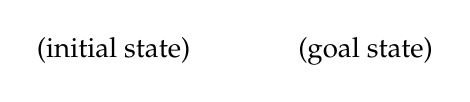
\begin{tikzpicture}
  % Initial state
  \node[align=center] at (7,-0.3) {(initial state)};
  \drawCube{7}{0.5}{0}{R}{red}{0.7}
  \drawCube{7}{1.2}{0}{B}{blue}{0.7}
  \drawCube{7}{1.9}{0}{G}{green}{0.7}

  % Goal state
  \node[align=center] at (10.2,-0.3) {(goal state)};
  \drawCube{10}{0.5}{0}{G}{green}{0.7}
  \drawCube{10}{1.2}{0}{B}{blue}{0.7}
  \drawCube{10}{1.9}{0}{R}{red}{0.7}
\end{tikzpicture}
\label{fig:intro-blocks}
\end{figure}

Planners are software systems specifically designed to find plans for planning tasks. Planners that do not rely on reasoning about SAT formulas may use several algorithms and techniques to explore the search space of possible operators and states in order to find an optimal or satisfactory plan, and typically take as input a formal representation of the planning problem, including the initial state, goal condition, and a set of available operators. The formal representation of a planning task can be specified using various notations~(\cref{sec:background-planning-notation}).


\section{Heuristic Search}
\label{sec:intro-heuristic-search}
Most planners are based on a best-first search algorithm such as greedy best-first search (GBFS)~\cite{Doran.Michie/1966}. GBFS arranges states in a priority queue based on their cost-to-goal estimate (also known as heuristic value or $h$-value) provided by the heuristic function. It first expands states with the lowest cost-to-goal estimate to find a solution. Various domain-independent heuristics effectively calculate the cost-to-goal estimate of a state by using domain logic, which has information that permits reasoning about operators and other rules, such as mutual exclusive relations (mutexes) that indicate infeasible states. These heuristics are based mainly on techniques such as abstractions~\cite{Culberson.Schaeffer/1998}, delete relaxation~\cite{Hoffmann.Nebel/2001}, and landmarks~\cite{Hoffmann.etal/2004,Helmert.Domshlak/2009}. The heuristic function is the most important component of a planner since it guides the search.


\section{Preferred Operators}
\label{sec:intro-preferred-ops}
Operators considered advantageous for specific reasons, such as generating states closer to the goal, are referred to as preferred operators~\cite{Helmert/2006,Richter.Helmert/2009}. These operators are used alongside heuristic functions to assist planners in minimizing the number of expanded states when solving a planning task.
By prioritizing the expansion of states generated by preferred operators, planners benefit from additional guidance, often resulting in a higher success rate for solving tasks than relying only on the heuristic function. Learning preferred operators shares similarities with learning policies, as both involve selecting actions more likely to result in desirable outcomes. The existing methods for identifying preferred operators are currently limited to logic-based approaches. The current most effective method uses the preferred operators calculated alongside the Fast-Forward (FF) heuristic~\cite{Hoffmann.Nebel/2001}, as implemented in the Fast Downward planning system~\cite{Helmert/2006}. Planners incorporating preferred operators emerged as winners in the satisficing track of the International Planning Competition (IPC) in the years 2004~\cite{Helmert/2006}, 2008~\cite{Richter.lama.etal/2010}, 2011~\cite{Richter.lama.etal/2011}, and 2018~\cite{Seipp-fast.etal/2018}.


\section{Learning with Neural Networks}
\label{sec:intro-deep-learning}
Learning with NNs refers to a machine learning approach that involves designing and training interconnected layers of artificial neurons, known as neural networks, inspired by the biological brain.
It involves learning hierarchical representations of data, where each layer in the network progressively extracts more complex and abstract features. Through the usage of NNs, learning algorithms can automatically discover and capture patterns from large-scale datasets in various tasks, including image classification, speech recognition, and natural language processing.

Learning models based on NNs can learn in different ways. This study focuses on supervised learning, which uses labeled datasets to classify or make predictions. In this case, a dataset used to train an NN can be represented as multiple pairs in the format $(y, x)$. The target $y$ refers to the desired output or label associated with a specific input instance $x$. With supervised learning, an NN can effectively learn and generalize from the provided labeled data to make accurate predictions or classify new, unseen inputs.


\section{Learning in Planning}
\label{sec:intro-learning-planning}
In recent years, interest in using NNs to learn heuristic functions~\cite{Ferber.etal/2020a,Yu.etal/2020,Shen.etal/2020,Ferber.etal/2022,OToole/2022,Bettker.etal/2022} or policies~\cite{Toyer.etal/2018,Toyer.etal/2020,Stahlberg.etal/2022} to solve planning tasks has increased. The general approach for supervised methods is to generate a set of samples as pairs of states and cost-to-goal values and use them for training an NN. However, it is challenging to learn effective heuristic functions since state spaces tend to grow exponentially in size as the amount of information needed to describe them increases, but the portion of the state space that we can actually sample is relatively small. Also, logic-based heuristics can be applied to any domain, while learned heuristics depend on the learning model, and even with domain-independent models, transfer learning can be difficult~\cite{Shen.etal/2020}. Moreover, learned heuristics are generally slow to compute, thus they need to be more informed, i.e., expand fewer states when compared to logic-based heuristics to reach the goal. These characteristics also apply to learning preferred operators.

\section{Contributions}
\label{sec:intro-contributions}
This study represents the first attempt to discover preferred operators from a sample set and use an NN to learn them. We present a new sampling method and a novel sample-based technique for identifying preferred operators. The technique involves backward search from the goal condition (also known as regression), constructing a graph with sampled states representing their successor-predecessor relationships, and determining the operators used to reach the goal condition as preferred operators for each state. We show that an NN can learn the preferred operators from a subset of the state space and effectively extend this learning to the entire state space across diverse planning domains. Furthermore, the proposed approach outperforms the current best logic-based preferred operator method in the benchmark tasks. In particular, this work presents:

\begin{itemize}
\item A novel method based on shortest path graphs to discover preferred operators in an existing sample set~(\cref{sec:sample-discovered-po}).
\item A new sampling method tailored for discovering preferred operators~(\cref{sec:sample-learn-po}).
\item An analysis of the quality of the learned preferred operators and a comparison to existing logic-based methods~(\cref{cha:exp-experiments}).
\end{itemize}
%
% - - - - - - - - - - - - - - - -- - - - - -
% background
% - - - - - - - - - - - - - - - -- - - - - -
% these are all things that exist already
% and that the reader needs to know before
%
\chapter{Background}
\label{cha:background}
This chapter provides essential information for comprehending the subsequent chapters of this work.


\section{Classical Planning Notation}
\label{sec:background-planning-notation}
In this section we present two ways to represent a classical planning task. The first one, STRIPS~\cite{Fikes.Nilsson/1971}, represents a planning task using propositional facts (Boolean variables). The second way, \sas~\cite{Backstrom.Nebel/1995}, represents a planning task using multi-valued state variables. %The third way, PDDL~\cite{Ghallab.etal/1998}, is based on predicate logic and is commonly used for writing planning tasks to be used as input for planners.

\subsection{STRIPS}
\label{sec:background-strips}

\begin{definition}[STRIPS Planning Task]\label{def:strips}
A planning task in STRIPS representation is defined by~$\Pi=\langle\mathcal{F},\mathcal{O},s_{0},s^{*}\rangle$, where~$\mathcal{F}$ has all the possible facts (propositions) that can be used to describe a state, $\mathcal{O}$~is a set of operators,~$s_{0} \subseteq \mathcal{F}$ is an initial state, and~$s^{*} \subseteq \mathcal{F}$ is the goal condition that specifies the facts that should be true to solve the task.
A state $s$ is defined as $s \subseteq \mathcal{F}$, where each fact in $s$ can be true ($f \in s$) or false ($f \notin s$). %The set~$\mathcal{S}$ of all states over $\mathcal{P}$ is the state space.
An operator~$o \in \mathcal{O}$ is defined by a triple~$\langle\pre(o),\add(o),\del(o)\rangle$ that specifies its precondition, add-effects and delete-effects, respectively, which are denoted as sets of facts.
\end{definition}

In STRIPS, we say that operator $o$ is applicable to state $s$ if its preconditions are satisfied by $s$, i.e., $\pre(o) \subseteq s$, and produces a successor state~$s' = \sucs(s,o) = (s \setminus \del(o)) \cup \eff(o)$. In other words, we progress a state $s$ with operator $o$ by setting the propositions in $\del(o)$ to false and in $\add(o)$ to true. The set of successor states of $s$ is denoted by~$\sucs(s)=\{\sucs(s,o)\mid o\in \mathcal{O}, \pre(o) \subseteq s\}$.

STRIPS formulas use conjunction of propositions with logical connectives (AND, OR, NOT) to express compound preconditions and effects. Also, STRIPS has no negated preconditions, and it is not possible to directly specify conditional effects, where the effect of an action depends on the initial state. However, we can simulate conditional effects by creating new operators in the planning task.

\begin{definition}[Plan]\label{def:plan}
A sequence of operators~$\pi=(o_1,\ldots,o_k)$ is valid for a state~$s_0$ if produces a sequence of states~$s_1,\ldots,s_k$ such that $s_i=\sucs(s_{i-1},o_i)$. A sequence~$\pi$ for the initial state~$s_{0}$ is called a plan if $s^{*} \subseteq s_{k}$. The plan length is defined as $|\pi|$. Among all the valid plans, the one with the minimum length is referred to as an optimal plan $\pi^{*}$. An optimal plan is the shortest plan that successfully achieves the goal condition from the initial state. Since in this work we only consider unitary cost operators, the plan cost is equal to the plan length.
\end{definition}

Heuristics based on delete-relaxation obtain the heuristic from a \emph{relaxed} version of the planning task. A relaxed planning task in STRIPS is defined as $\Pi^{+}=\langle\mathcal{P},\mathcal{O'},s_{0},s^{*}\rangle$, where $\mathcal{O'} = \{ \langle \pre(o), \add(o), \emptyset \rangle \,|\, o \in O \}$, i.e., the delete-effects of the planning task are ignored. Relaxed tasks can be solved efficiently even though finding the optimal solution is $\mathcal{NP}$-hard~\cite{Bylander/1994}. For example, the heuristic \hadd approximates the perfect heuristic value for a state $s$ as the sum of the costs of achieving each proposition in $s^{*}$ independently of the others.

\subsection{\sas}
\label{sec:background-sas}
We also use the \sas representation to describe classical planning tasks independent of any particular domain. \sas shares similarities with STRIPS, but it allows state variables to have an arbitrary and potentially non-binary finite domain. These multi-valued variables can express mutexes that are not explicitly recognized in STRIPS. Suppose we have a planning task with a robot in a grid with $n$ possible locations it needs to visit. With STRIPS, we need $n$ facts to indicate all the possible locations where the robot can be, and the STRIPS representation does not explicitly capture the mutex that the robot cannot exist in multiple locations simultaneously. In \sas, this information can be naturally expressed using a single multi-valued variable for the location of the robot. The variable has a finite domain consisting of the $n$ possible locations, enforcing that the robot can only occupy one location at a time. Thus, only one proposition from the $n$ possibilities can be true in any state.

\begin{definition}[\sas Planning Task]\label{def:sas}
A \sas task is defined as $\Pi=\langle\mathcal{V},\mathcal{O},s_0,s^*\rangle$, where $\mathcal{V}$ is a set of state variables, and each variable $v\in \mathcal{V}$ has a finite domain~$\dom(v)$, that represents the possible mutually exclusive values of each variable, $\mathcal{O}$ is a set of operators where each operator $o \in \mathcal{O}$ is defined as a pair of preconditions and effects $(\pre(o),\eff(o))$, both partial states~$s$ defined as a partial function $s:\mathcal{V}\rightarrow \mathcal{D}$, where $\mathcal{D}=\cup_{v\in \mathcal{V}}\dom(v)$, such that $s(v)\in \dom(v)$ whenever $s(v)$ is defined. Otherwise, $s(v)$ is undefined and written as $s(v)=\bot$. Given a partial state $s$, $var(s) \in \mathcal{V}$ is a finite set which lists all variables assigned in $s$. A (complete) state $s$ is a partial state defined on all variables in~$\mathcal{V}$, i.e, $var(s) = \mathcal{V}$. The state~$s_0$ defines the initial state, and the partial state~$s^*$ defines the goal condition.
\end{definition}

An operator $o \in \mathcal{O}$ is applicable to a state $s$ if its preconditions are fulfilled by $s$, denoted by $s \subseteq \pre(o)$, and it generates a successor state $s'=\sucs(s,o):=\eff(o)\circ s$. Here, $s'=t\circ s$ is defined as $s'(v)=t(v)$ for all $v$ such that $t(v)$ is defined, and for all other cases, $s'(v)=s(v)$. The set of all successor states resulting from state $s$ is denoted by $\sucs(s)=\{{\sucs(s,o)\mid o\in \mathcal{O}, s \subseteq \pre(o)}\}$. A state variable can never be made undefined once made defined by an operator.
% A sequence of operators $\pi=(o_1,\ldots,o_k)$, where $o_i\in \mathcal{O}$, is considered valid for the initial state $s_0$ if, for $i\in[k]$, operator $o_i$ can be applied to $s_{i-1}$, and produces $s_i=\sucs(s_{i-1},o_i)$. %A plan refers to a valid sequence $\pi$ for $s_0$ such that $s^* \subseteq s_k$. In this work, all operators have unit costs, so the plan length is $|\pi| = k$.
%If $s$ is a partial state, it would be incorrect to write $\pre(o) \subseteq s$. The expression $\pre(o) \subseteq s$ implies that the preconditions of the operator $o$ are fully satisfied by the state $s$. It is likely that $s$ only contains a subset of the conditions specified in $\pre(o)$.

Planners typically convert an input task in STRIPS to~\sas or an equivalent multi-valued representation. We can represent planning tasks in STRIPS using~\sas by converting each fact to a state variable with domain true and false. On the other hand,~\sas can be represented in STRIPS by converting each possible variable assignment to a fact. Note that \sas supports partial assignments while STRIPS assumes all states are complete (unmentioned facts are considered false).
Also,~\sas tasks are more concise than STRIPS tasks. In STRIPS, if we have $n$ facts, the size of the set of states would be $2^n$. In~\sas, with $n$ variables, the size of the set of states would be $dom(v_{1}) \times dom(v_{2}) \times \ldots \times dom(v_{n})$.

%\subsection{PDDL}
%\label{sec:background-pddl}
%We can also represent a classical planning task using PDDL. Tasks specified in PDDL are written in a Lisp-like syntax and are separated into two definitions, the domain, which specifies the operators and predicates, and the task, which specifies the objects, the initial state, and the goal condition. The following definitions describe a restricted version of PDDL that encodes STRIPS-like planning tasks.

%\begin{definition}[PDDL Domain]\label{def:pddl-domain}
%A PDDL domain is defined as a tuple $D = (\mathcal{P}, \mathcal{O})$, where $\mathcal{P}$ is a set of predicates representing the state of the world. Each predicate $p \in \mathcal{P}$ can be true or false in a given state. The set of operators is defined as $\mathcal{O}$. Each operator $o \in \mathcal{O}$ has a pre-condition $\pre(o)$ and an effect $\eff(o)$.
%\end{definition}

%In PDDL, effects are not explicitly separated into add-effects and delete-effects, instead, delete-effects are represented by negating the predicates.

%\begin{definition}[PDDL Task]\label{def:pddl-domain}
%A PDDL task is a triple $T = (D, s_{0}, s^{*})$, where $D$ is the domain definition associated with the problem, $s_{0}$ is the initial state, represented as $s_{0} = \{p_1, p_2, \ldots, p_n\}$, where $p_i \in \mathcal{P}$, and $s^{*}$ is the goal condition, denoted as $s^{*} = \{q_1, q_2, \ldots, q_m\}$, where $q_i \in \mathcal{P}$ represents the desired state of predicate $q_i$ to be achieved.
%\end{definition}

%Actions represent the possible operations or transformations that can be performed, while predicates describe the properties or conditions that can be true or false within the domain. Objects are the entities involved in the planning task, while the initial state describes the starting configuration or state of the objects. The goal condition defines the desired state that a planner aims to achieve.

%As an example, consider Blocks World, where $(ontable~?x)$ represents a predicate that indicates if a block $x$ is on the table or not, and $(pickup~?x)$ is an action that defines the act of picking up block $x$. This action is further specified by a set of preconditions $(and~(clear~?x)~(ontable~?x)~(handempty))$ that must hold true before $(pickup~?x)$ is applied, i.e., $x$ must be clear (no other block above it), $x$ must be on the table, and the hand must be empty. The effects of applying $(pickup~?x)$ are $$(and~(not~(ontable~?x))~(not~(clear~?x))~(not~(handempty))~(holding~?x)),$$

%that is, $x$ is not on the table, $x$ is not clear, the hand is not empty, and the hand is holding $x$.

\section{Regression}
\label{background-regression}

The predecessor of a partial state $s$ under operator $o$, denoted $\pred(s,o)$, can be obtained through a process called backward search or regression. Regression involves determining predecessor states that can lead to the current partial state by applying the operator $o$. An operator $o$ is considered relevant for partial state $s$ if $\eff_r = \dom(\eff(o)) \cap \dom(s) \neq \emptyset$, i.e., at least one defined effect in $o$ overlaps with $s$, and consistent if $s \subseteq \eff(o)|_{\eff_r}$, i.e., the operator agrees with the defined effects in $s$. An operator $o$ is said to be \emph{backward applicable} in partial state $s$ if it is both relevant and consistent with $s$, and it leads to a predecessor $r$ given by $r=\pre(o)\circ (s|_{\dom(s)\setminus\eff_r})$. Also, $s \subseteq \sucs(r,o)$ can differ from $s$, i.e., applying an operator to a predecessor state may result in a subset of the current partial state, but it does not necessarily cover all the possible states represented by $s$.
% $(s|_{\dom(s)\setminus\eff_r})$: This part refers to the restriction or projection of the current partial state $s$ onto the variables in its domain ($\dom(s)$) that are not affected by the effects of operator $o$ ($\eff_r$). In other words, it selects the values of the variables in $s$ that are not modified by $o$.
A partial state $s$ has predecessors $\pred(s)=\{{\pred(s,o)\mid o\in \mathcal{O}}\}$ where $o$ is backward applicable to $s$, and a regression sequence from state $s_0$ is valid if $o_i$ can be applied to $s_{i-1}$ and produces $s_i=\pred(s_{i-1},o_i)$. All partial states~$s_k$ can reach a partial state $s_{0} \subseteq s$ in at most $k$ forward applications of the reversed operator sequence.
If a valid regression sequence $\rho = (o_1, \ldots, o_k)$ is generated, it will produce a sequence of partial states that can reach the goal condition $s^*$ within a maximum of $k$ steps.


\section{State Spaces}
\label{background-state-spaces}
Let $S$ be a set of states, $s_0 \in S$ be an initial state, $s^{*} \in S$ be the goal condition, and $\sucs : S \to 2^S$ be a successor function, which maps each state to a set of possible successor states and determines the available transitions. A state space is a tuple $\spp=\langle S, s_0, s^{*}, \sucs \rangle$.
\begin{definition}[State Space of $\Pi$]
For any planning task $\Pi$ with states $S$, initial state $s_0$, goal condition $s^{*}$, and successor function $\sucs$, the corresponding state space of $\Pi$ is denoted as $\spp(\Pi) = \langle S, s_0, s^{*}, \sucs \rangle$.
\end{definition}

The forward state space (\fsp) refers to the set of states that can be reached from the initial state $s_0$ by applying the successor function $\sucs$ in the forward direction. It represents the states that can be reached forward from the initial state towards the goal condition.

\begin{definition}[Forward State Space of $\Pi$]
The forward state space for a planning task $\Pi$ is denoted as $\fsp(\Pi) = \langle S_{\text{F}}, s_0, s^{*}, \sucs \rangle$, where $S_{\text{F}}$ is the set of states reachable from the initial state, and $\sucs : S_{\text{F}} \to 2^{S_{\text{F}}}$ is the successor function that maps each state to a set of possible successor states and determines the available transitions in the forward direction.
\end{definition}

In other words, $\fsp(\Pi)$ is defined as the subset of states and transitions within $\spp$ that are relevant to the planning task $\Pi$ and the forward expansion towards the goal condition. States from the \fsp are expanded when solving a task, for example by using a best-first search algorithm.

The backward state space (\bsp), on the other hand, refers to the set of states that can be reached from the goal condition $s^{*}$ by applying a predecessor function $\pred$. It represents the states that can be reached backward from the goal condition towards the initial state (regression).

\begin{definition}[Backward State Space of $\Pi$]
The backward state space of a planning task $\Pi$ is denoted as $\bsp(\Pi) = \langle S_{\text{B}}, s_{0}, s^{*}, \pred \rangle$, where $S_{\text{B}}$ is the set of states reachable from the goal condition and $\pred : S_{\text{B}} \to 2^{S_{\text{B}}}$ is a predecessor function that maps each state to a set of possible predecessor states and determines the available transitions in the backward direction.
\end{definition}


\section{Heuristic Functions}
\label{sec:background-heuristics}
A heuristic function $h:\mathcal{S}\rightarrow \mathbb{R}^{\geq 0}\cup\{\infty\}$ estimates the optimal plan length from a state $s$ to the goal $s^*$, where the perfect heuristic function is defined as $\hstar(s) = |\pi_{s}^{*}|$, i.e., the length of the optimal plan from $s$ to $s^{*}$. Heuristic functions are used to guide search algorithms, optimization techniques, or decision-making processes by providing informed estimates or approximations based on available information or problem-specific knowledge. The goal of a heuristic function is to efficiently guide the search or decision-making process towards more promising paths or solutions, even in the absence of complete or perfect information. A heuristic function can have several properties that indicate its quality, such as:

\begin{itemize}
\item Admissibility: $h(s) \le \hstar{(s)}$, i.e., the heuristic never overestimates the true cost-to-goal.
\item Consistency (or monotonicity): $h(s) \le h(s') + cost(o)$ for all transitions from a state $s$ to a successor $s'$, i.e., $s \xrightarrow{o} s'$, where $cost(o)$ is the cost of applying operator $o$ to reach $s'$ from $s$.
\item Goal-awareness: $h(s) = 0$ for all goal states.
\item Safeness: $h(s) = \infty$ implies $\hstar (s) = \infty$, for example in dead-ends.
\end{itemize}

Heuristics are typically derived from a model of the task, such as the \sas model introduced earlier, but can also be obtained by learning the map of some state $s$ to its heuristic value $h(s)$, where the desired output of the NN can be either the direct cost-to-goal estimates or some form of encoding representing these estimates.

In this study, we use a propositional representation of a state to learn heuristic functions and preferred operators~\cite{Ferber.etal/2020a,Yu.etal/2020,Ferber.etal/2022,OToole/2022,Bettker.etal/2022}. We use the notation from~\citet{Bettker.etal/2022}.
Consider a planning task $\Pi=\langle\mathcal{V},\mathcal{O},s_0,s^*\rangle$, where $\mathcal{V}=\{v_1,\ldots,v_n\}$ is a set of variables, and $D(v_i)=\{d_{i1},\ldots,d_{i,s_i}\}$ the domains of variable $v_i$, where $i\in[n]$.
A state $s$ is represented as a sequence of facts $\mathcal{F}(s)=(f_{11},f_{12},\ldots,f_{1,s_1},\ldots,f_{n1},f_{n2},\ldots,f_{n,s_n})$. Each fact $f_{ij}=[s(v_i)=d_{ij}]$ corresponds to a variable $v_i$ taking on a specific value $d_{ij}$ in state $s$. If the variable $v_i$ has the assigned value $d_{ij}$ in state $s$, then the fact $f_{ij}$ is considered true.
The facts $\mathcal{F}_{i}=\{f_{i1},\ldots,f_{i,s_i}\}$ associated with variable $v_i$ must adhere to the consistency condition $\sum_{f\in \mathcal{F}i} f\leq 1$. This means that each variable can take at most one value. When $v_i$ is undefined, $\sum_{f\in \mathcal{F}_i} f=0$.

For example, let $\mathcal{F}$ be a set of facts, and let $f_i, f_j \in \mathcal{F}$ be two facts. We say that $f_i$ and $f_j$ are mutex if $\neg(f_i \land f_j)$ holds, i.e., $f_i$ and $f_j$ cannot both be true at the same time in any valid state of the planning problem.
We use the notation $\mutex(\mathcal{F})$ to denote when the constraint $\sum_{f\in \mathcal{F}} [f]\leq 1$ must be satisfied for the states of the planning task.


\section{Greedy Best-First Search}
\label{sec:background-gbfs}
Greedy Best-First Search (GBFS, \cref{alg:gbfs}) is a best-first search algorithm typically used by planners to solve planning tasks by expanding the \fsp. GBFS organizes states in a priority queue based on their cost-to-goal estimate, which is determined by a heuristic function $h$. GBFS expands states with the \emph{lowest} cost-to-goal estimate first in order to find a solution. Unlike the \astar algorithm~\cite{Hart.etal/1968}, GBFS does not consider the cost of the path taken ($g$-value). This makes GBFS efficient when the heuristic function is accurate, but it sacrifices optimality guarantees, whereas~\astar is optimal when the heuristic used is both admissible and consistent.

\begin{algorithm}[tb]
\caption{Greedy best-first search}
\label{alg:gbfs}
\begin{algorithmic}[1]
\Procedure{GBFS}{$s_{0}, s^{*}, h$}
  \State $Q \gets$ priority queue ordered by lowest $h$
  \If{$h(s_{0}) < \infty$}
    \State Insert $s_0$ into $Q$ with priority $h(s_0)$
    \State Mark the initial state $s_0$ as visited
  \EndIf

  \While{$Q$ is not empty}
    \State $s \gets$ state with the highest priority in $Q$
    \State Remove $s$ from $Q$

    \If{$s$ satisfies the goal condition $s^{*}$}
      \State \textbf{return} the solution
    \EndIf

    \State $S' \gets \{s' \mid s' \in succ(s)\}$
    \ForAll{successor states $s' \in S'$}
      \If{$s'$ has not been visited \textbf{and} $h(s') < \infty$}
        \State Mark $s'$ as visited
        \State Insert $s'$ into $Q$ with priority $h(s')$
      \EndIf
    \EndFor
  \EndWhile

  \State \textbf{return} failure (no solution found)
\EndProcedure
\end{algorithmic}
\end{algorithm}

\section{Preferred Operators}
\label{sec:background-preferred-operators}

Preferred operators can be described as operators that, given a particular state $s$, tend to generate successors more likely to satisfy the goal condition when compared to other successors of $s$. Preferred operators provide a way to prioritize the expansion of certain states over others during the search. Although the method of identifying preferred operators varies,~\citet{Hoffmann.Nebel/2001} introduced the first approach in the original Fast-Forward (FF), where preferred operators are calculated alongside the FF heuristic.
Specifically, the FF planner computes a relaxed planning graph~(\cref{alg:computing-rpg}) that represents the relaxed task, i.e., ignoring delete-effects. From the relaxed planning graph, FF extracts the relaxed plan~(\cref{alg:extracting-relaxed-plan}) with its length as the cost-to-goal estimate for a state $s$. To extract the relaxed plan, the algorithm marks the goal facts that need to be achieved at each layer $k$ of the relaxed planning graph, then iterate from the last layer to the initial layer, marking the actions at layer $k$ that achieve the goal facts of the same layer. The preferred operators, then called \emph{helpful actions}, are defined as the set $\{o \mid pre(o) \subseteq s, add(o) \cap S_{k=1}^{*} \neq \emptyset \}$, where $S_{k=1}^{*}$ denotes the set of goal facts at layer $1$ of the relaxed plan. In summary, the preferred operators of the FF planner are a subset of all possible operators that satisfy two conditions: they can be applied given the current state and contribute to achieving at least one goal fact at the first layer of the relaxed plan.

In the original implementation of the FF planner, the preferred operators prune the search space and only evaluate successors generated via preferred operators. However, this makes the search incomplete~\cite{Richter.Helmert/2009}, i.e., it does not guarantee a solution or determine if there is none, and FF restarts without preferred operators if they fail.\footnote{\cref{alg:computing-rpg,alg:extracting-relaxed-plan} were modified from~\citet{Wickler.etal/2015}.}

\begin{algorithm}[tb]
\caption{Computing the relaxed planning graph}
\label{alg:computing-rpg}
\begin{algorithmic}[1]
\Procedure{RelaxedPlanningGraph}{relaxed planning task $\Pi^{+}$}
  \State $P_{0} \gets s_{0}$ \textcolor{gray}{\# \emph{Initial proposition layer}.}
  \State $k \gets 0$ \textcolor{gray}{\# \emph{Index of the current layer}.}
  \While{$s^{*} \nsubseteq P_{k}$}
    \State $k \gets k + 1$
    \State \textcolor{gray}{\# \emph{Computes the action layer $O_{k}$ at layer $k$, i.e., all the actions}}
    \State \textcolor{gray}{\# \emph{with the preconditions satisfied in the layer $P_{k}$}.}
    \State $O_{k} \gets \{o \in O\ \mid pre(o) \subseteq P_{k}\}$
    \State $P_{k} \gets P_{k-1}$
    \ForAll{$o \in O_{k}$}
      \State \textcolor{gray}{\# \emph{Computes the proposition layer $P_{k}$ at layer $k$}.}
      \State $P_{k} \gets P_{k} \cup add(o)$
    \EndFor
    \If{$P_{k} = P_{k-1}$}
      \State \textbf{return} failure
    \EndIf

  \EndWhile

  \State $G^{+} \gets $ [$P_{0}, O_{1}, P_{1},\ldots,O_{k}, P_{k}$] \textcolor{gray}{\# \emph{The relaxed planning graph}.}
  \State \textbf{return} $G^{+}$
\EndProcedure
\end{algorithmic}
\end{algorithm}

\begin{algorithm}[tb]
\caption{Extracting the relaxed plan}
\label{alg:extracting-relaxed-plan}
\begin{algorithmic}[1]
\Procedure{RelaxedPlan}{relaxed planning graph $G^{+}$, goal facts $s^{*}$}
  \State $P \gets$ proposition layers of $G^{+}$
  \State $O \gets$ action layers of $G^{+}$
  %\State $l \gets$ number of layers in $G^{+}$
  %\If{$s^{*} \nsubseteq P_{l}$}
  %  \State \textbf{return} failure
  %\EndIf
  \State $plan \gets \emptyset$
  \State \textcolor{gray}{\# \emph{firstlayer($x$,$y$) returns the number of the first layer at which $x$ appears in $y$.}}
  \State \textcolor{gray}{\# \emph{M = maximum(index of the first layer where each fact of $s^{*}$ first appears in $P$).}}
  \State $M \gets$ $\max \{\text{firstlayer}(s_{i}^{*}, P) \mid s_{i}^{*} \in s^{*}\}$
  \For{$k \gets 0$ \textbf{to} $M$}
    \State \textcolor{gray}{\# \emph{$S_{k}^{*}$ are the goal facts that need to be achieved in $P_{k}$.}}
    \State $S_{k}^{*} \gets$ $\{s_{i}^{*} \in s^{*} \mid \text{firstlayer}(s_{i}^{*}, P_{k}) = k\}$
  \EndFor
  \For{$k \gets M$ \textbf{to} $1$}
    \ForAll{$s_{k}^{*} \in S_{k}^{*}$}
      \State \textcolor{gray}{\# \emph{Selects the action $o$ that achieves the goal fact $s_{k}^{*}$}}
      \State \textcolor{gray}{\# \emph{and appears for the first time in layer $k$}.}
      \State $o \gets$ $\text{firstlayer}(o, O_{k}) = k \mid s_{k}^{*} \in add(o)$
      \State $plan \gets plan \cup \{o\}$
      \State \textcolor{gray}{\# \emph{Now add the preconditions of $o$ as sub-goals to $S^{*}$}}
      \State \textcolor{gray}{\# \emph{in the layer where $p$ first appears}.}
      \ForAll{$p \in pre(o)$}
        \State $S_{firstlayer(p, P)}^{*} \gets S_{firstlayer(p, P)}^{*} \cup \{p\}$
      \EndFor
    \EndFor
  \EndFor
  \State \textbf{return} $plan$
\EndProcedure
\end{algorithmic}
\end{algorithm}

The current approach to extract preferred operators is the one implemented in the Fast Downward planning system~\cite{Helmert/2009}, based on domain transition graphs, compatible with \sas, instead of planning graphs as previously described, where the preferred operators obtained with the calculation of the FF heuristic are the current best.
% A DTG is defined as follows.
%Let $\Pi = \langle \mathcal{V}, \mathcal{O}, s_0, s^* \rangle$ be a \sas planning task, and let $v \in \mathcal{V}$. The DTG of variable $v$ is the labeled directed graph $\text{DTG}(v, \Pi)$ with vertices $D_v$ and an arc $(d, d')$ labeled with operator $o \in \mathcal{O}$ whenever either $\pre_{o}(v) = d$ and $\eff_{o}(v) = d'$, or $\pre_{o}(v)$ is undefined and $\eff_{o}(v) = d'$. We refer to $(d, d')$ as a value transition of $v$. We write $d \xrightarrow{o} d'$ if there exists an operator $o$ that can modify the value of $v$ from $d$ to $d'$.
%To summarize, the DTG of a variable $v$ shows all the possible values of $v$ as vertices, and the arcs with their corresponding operators represent the transitions between those values. Furthermore, in Fast Downward, ignoring delete-effects in a multi-valued task is equivalent to assume that each state variable can hold several values simultaneously.
Fast Downward extends the traditional GBFS algorithm to support preferred operators and ensure completeness. This is achieved by introducing a dual-queue approach: the ``default queue'' receives all generated states (default behavior without preferred operators), while the ``preferred queue'' only accepts states generated by preferred operators. Expansion of states occurs alternately from both queues or may use boosting~\cite{Richter.Helmert/2009}.
With a boost value $n$, when a state with a lower $h$-value than any previously expanded state is encountered during the search (meaning the search progresses) the preferred queue is used for the next $n$ expansions, as long as it has elements. The boost value is cumulative, so each time the search progresses, $n$ expansions are added to the remaining number of subsequent expansions from the preferred queue.
% With a boost value $n$, if the search expands a state with an $h$-value lower than all previously expanded states (indicating progress in the search), the preferred queue is used for the subsequent $n$ expansions, as long as it contains elements. Furthermore, the boost value is cumulative, meaning that whenever the search progresses, $n$ expansions are added to the remaining number of subsequent expansions from the preferred queue.

In Fast Downward, the first expansion of the search is always from the default queue, so even if we have preferred operators that always generate a successor closest to the goal, the plan may not be optimal if the heuristic is inaccurate. Also, there are cases where a preferred operators generates a successor state that has already been generated. Consequently, the state is not added to the preferred queue, which means it cannot be expanded first (as the preferred queue has higher priority), and another state, potentially further from the goal, is expanded instead.

\section{Neural Networks}
\label{sec:background-neural-nets}

A multi-layer perceptron is a commonly used NN architecture comprising an input layer, one or more hidden layers, and an output layer. The neurons within the hidden layers apply activation functions to the weighted sum of their inputs, which introduces both linear and nonlinear transformations. A bias term represents a constant value that is optionally added to the weighted sum of inputs of a neuron before applying the activation function, introducing an offset in the activation that allows the NN to account for any systematic errors or deviations in the data. The weights and biases of the neurons are learned through a process called backpropagation, which optimizes a loss function using gradient descent or its variations. For more information on backpropagation and gradient descent, refer to~\citet{Goodfellow.etal/2016}.

The mean squared error (MSE) loss function is commonly used for regression problems, where the goal is to predict continuous values.
\begin{definition}[Mean Squared Error]\label{def:mse}
Given a prediction $\hat{y}$ and the corresponding target value $y$, the MSE loss is calculated as the mean of the squared differences between the prediction and the target:

$$\text{MSE}(\hat{y}, y) = \frac{1}{N} \sum_{i=1}^{N} (\hat{y}_i - y_i)^2,$$

where $\hat{y}_i$ represents the $i$-th element of the prediction vector $\hat{y}$, $y_i$ represents the $i$-th element of the target vector $y$, and $N$ is the total number of elements in the vectors.
\end{definition}

The binary cross-entropy (BCE) loss function is commonly used for binary classification problems, where the goal is to predict a binary outcome, or multi-label classification problems where there can be more than one correct outcome~\cite{Tsoumakas.etal/2007}.
\begin{definition}[Binary Cross-Entropy]\label{def:mse}
Given a prediction $\hat{y}$ and the corresponding binary target value $y$, the BCE loss is calculated as the average of the element-wise cross-entropy between the prediction and the target:

$$\text{BCE}(\hat{y}, y) = -\frac{1}{N} \sum_{i=1}^{N} \left[y_i \log(\hat{y}_i) + (1 - y_i) \log(1 - \hat{y}_i)\right],$$

where $\hat{y}_i$ represents the $i$-th element of the prediction vector $\hat{y}$, $y_i$ represents the $i$-th element of the target vector $y$, and $N$ is the total number of elements in the vectors.
\end{definition}

In this study, we use a feedforward NN with residual blocks.

\begin{definition}[Feedforward Neural Network]
Let us consider a feedforward NN with L layers. For simplicity, assume each layer has the same number of neurons, denoted by $N$. The input to the network is represented $x$, and the output is denoted by $y$. The activation function of a neuron in the $l$-th layer is denoted as $a^l(\cdot)$, and the weights connecting the $i$-th neuron in layer $l-1$ to the $j$-th neuron in layer $l$ are denoted as $w^{l}_{ij}$. The bias of the $j$-th neuron in layer $l$ is denoted as $b^{l}_{j}$. The output of the $j$-th neuron in layer $l$ is given by:

$$z^{l}_{j} = \sum_{i=1}^{N} w^{l}_{ij} a^{l-1}_{i} + b^{l}_{j}$$

The activation of the $j$-th neuron in layer $l$ is then computed as:

$$a^{l}_{j} = a^{l}(z^{l}_{j})$$
\end{definition}

\cref{fig:neural-network} shows an example of a simple fully-connected NN. Common activation functions include sigmoid, rectified linear units (ReLU), and tanh~(\cref{fig:activation-functions}).

\begin{figure}[tb]
\caption[A fully-connected neural network]{A neural network with $n$ input neurons, two hidden layers with $m$ neurons, and an output layer with $k$ neurons.}
\vspace{\baselineskip}
\centering
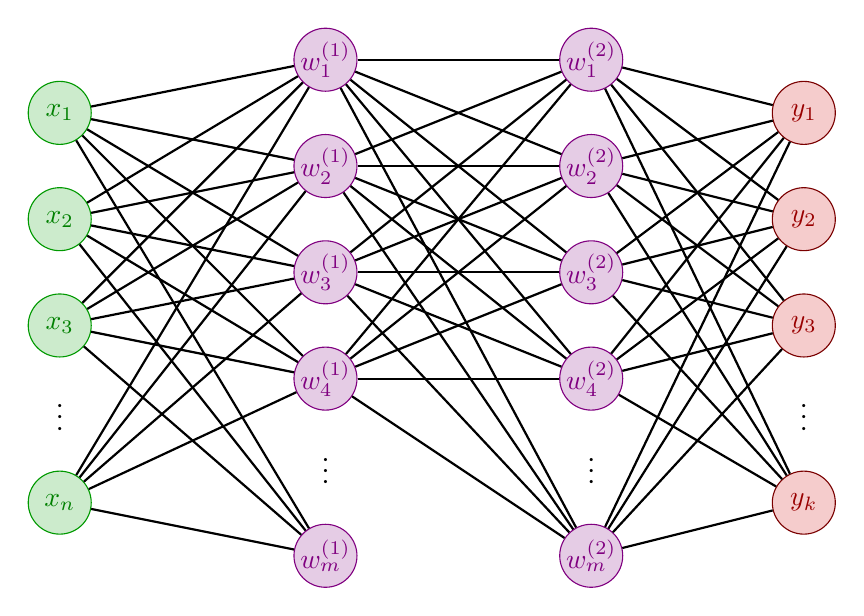
\begin{tikzpicture}[x=1.5cm,y=1.0cm,scale=0.9]

\foreach\i in {1,2,3}
  \node[input]  (x\i)  at (0,-1.5*\i)       {$x_\i$};
\node[input]    (x4)   at (0,-7)            {$x_n$};

\foreach\i in {1,2,3,4}
  \node[hidden] (w_1\i)  at (2.5,0.75-1.5*\i) {$w_\i^{(1)}$};
\node[hidden]   (w_15)   at (2.5,-7.75)       {$w_m^{(1)}$};

\foreach\i in {1,2,3,4}
  \node[hidden] (w_2\i)  at (5.0,0.75-1.5*\i) {$w_\i^{(2)}$};
\node[hidden]   (w_25)   at (5.0,-7.75)       {$w_m^{(2)}$};

\foreach\i in {1,2,3}
  \node[output]  (y\i)  at (7,-1.5*\i)       {$y_\i$};
\node[output]    (y4)   at (7,-7)            {$y_k$};

% connections
\foreach\i in {1,2,3,4,5} \foreach\j in {1,2,3,4}
{
  \draw[black,thick]   (w_1\i) -- (x\j);
  \draw[black,thick]   (w_2\i) -- (w_1\j);
  \draw[black,thick]   (w_2\i) -- (y\j);
}
% dots
\foreach\i/\j in {x3/x4,w_14/w_15,w_24/w_25,y3/y4}
  \node at ($(\i)!0.5!(\j)$) {\strut$\vdots$};
\end{tikzpicture}
\label{fig:neural-network}
\end{figure}

\begin{figure}[tb]
\caption[Common activation functions]{Sigmoid, ReLU, and tanh activation functions.}
\vspace{\baselineskip}
\centering
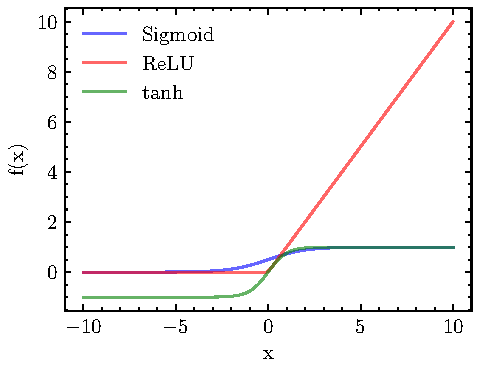
\includegraphics[scale=1.0]{img/sigmoid-relu-tanh}
\label{fig:activation-functions}
\end{figure}

The data ``feed'' to an NN is typically divided into two sets. The training dataset is used to train the model by adjusting its parameters based on input samples and corresponding target values. The validation dataset is used to evaluate the performance of the model and detect overfitting during training. Overfitting occurs when a model excessively fits the training data but fails to generalize to unseen data.

An epoch is an iteration of the entire training dataset. It involves feeding each training sample through the network, updating weights based on the loss function, and performing forward and backward propagation for all training samples.
Early stop, or patience, monitors a chosen metric (e.g., validation loss) and halts training if there is no improvement for a specified number of consecutive epochs. Early stopping prevents overfitting, enhances generalization, and preserves the performance of the model at the point of best validation metric.

\begin{definition}[Early Stop]
Let $M$ represent the chosen metric (e.g., validation loss) and $n$ denote the number of consecutive epochs without improvement allowed. Given the current epoch $t$, the training is stopped if the following condition is met:

$$M(t) > \min\{M(t-1), M(t-2), \ldots, M(t-n)\}$$

where $M(t)$ represents the metric value at epoch $t$.
\end{definition}

We can feed data to an NN during training in batches, which are subsets of training samples processed together in each epoch iteration.
This approach improves computational efficiency by allowing multiple samples to be processed simultaneously, rather than updating the network weights after processing each training sample (which is computationally inefficient).
Larger batch sizes enable efficient parallel processing but require more memory, while smaller batch sizes consume less memory but may result in slower training convergence due to more frequent weight updates.

Standard NNs may suffer from the vanishing gradient problem~\cite{Hochreiter/1991}. The gradients tend to diminish as they propagate backward through multiple layers, making it challenging for earlier layers to learn meaningful representations. This problem hampers the optimization process and restricts the overall performance of the network.

Residual Neural Networks (ResNets)~\cite{He.etal/2016} can reduce the vanishing gradient problem. ResNets use skip connections that bypass layers, allowing the information to flow directly from one layer to another. This bypassing mechanism mitigates the vanishing gradient problem and facilitates the training of deep networks.

\begin{definition}[Skip Connection]
Let us consider a ResNet architecture with $L$ layers. The output of the $l$-th layer is denoted by $a^{l}$, and the output of the previous layer is denoted by $a^{l-1}$. The residual connection between the $l$-th and $l-1$-th layers can be represented as:

$$a^{l} = a^{l-1} + \mathcal{F}(a^{l-1}, W^{l}),$$

where $\mathcal{F}$ represents a residual function, typically implemented as a fully connected layer, and $W^{l}$ denotes the learnable parameters of this function.
\end{definition}

\cref{fig:residual-block} has a visual representation of a small \emph{residual block} with a skip connection.

\begin{figure}[tb]
\caption[A residual block]{A residual block with two hidden layers.}
%\vspace{\baselineskip}
\centering
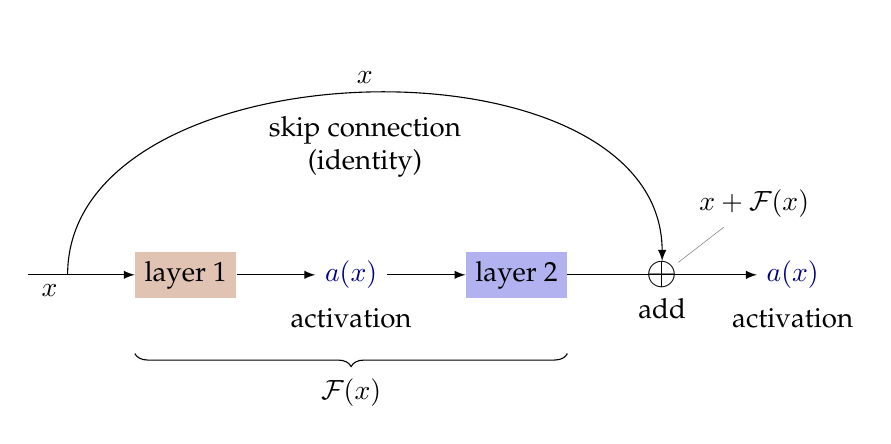
\begin{tikzpicture}[scale=1.0]
  \node[fill=myorange!30] (l1) {layer 1};
  \node[blue!50!black, right=of l1, label={below:activation}] (act1) {$a(x)$};
  \node[fill=myblue!30, right=of act1] (l2) {layer 2};
  \node[right=of l2, font=\Large, label={below:add}, inner sep=0, pin={60:$x + \mathcal F(x)$}] (add) {$\oplus$};
  \node[blue!50!black, right=of add, label={below:activation}] (act2) {$a(x)$};

  \draw[->] (l1) -- (act1);
  \draw[->] (act1) -- (l2);
  \draw[<-] (l1) -- ++(-2,0) node[below, pos=0.8] {$x$};
  \draw[->] (l2) -- (act2) node[above, pos=0.8] {};
  \draw[->] ($(l1)-(1.5,0)$) to[out=90, in=90] node[below=1ex, midway, align=center] {skip connection\\(identity)} node[above, midway] {$x$} (add);
  \draw[decorate, decoration={brace, amplitude=1ex, raise=1cm}] (l2.east) -- node[midway, below=1.2cm] {$\mathcal F(x)$} (l1.west);
\end{tikzpicture}
\label{fig:residual-block}
\end{figure}


\section{Learning Heuristic Functions}
\label{sec:related-h}
While prior research has not specifically addressed learning preferred operators, there have been several studies on using learning heuristic functions for classical planning. These studies can be categorized into two primary approaches.
The first approach heavily relies on domain logic to generate samples and instantiate networks. Its objective is to generalize across domains or a planning formalism.
On the other hand, the second approach minimally uses domain logic for generating samples and focuses on generalization within a state space.

The first approach uses structured NNs with architectures specifically designed to align with the characteristics and requirements of the given input task. Examples include learning domain-independent heuristic functions with hypergraph NNs~\cite{Shen.etal/2020}, and learning policies with action schema networks~\cite{Toyer.etal/2018,Toyer.etal/2020} and graph NNs~\cite{Stahlberg.etal/2022}. These approaches are generally applicable to state spaces that differ from the ones they were originally trained on. The major limitation of this set of approaches is that they heavily rely on domain logic, and can also have significant computational overhead, as in the case of action schema networks. Moreover, in domain-independent approaches such as hypergraph NNs, where the network can be applied to a different domain than the one it was originally trained on, the search performance is considerably inferior when compared to logic-based heuristics in terms of coverage (number of solved tasks within a given time limit).

The second approach uses supervised learning to train a feedforward NN with pairs of states and cost-to-goal estimates. Samples can be generated with forward search from the initial state~\cite{Ferber.etal/2020a}, backward search from the goal~\cite{Yu.etal/2020,OToole/2022,Bettker.etal/2022}, or a combination of both~\cite{Ferber.etal/2022}.
This set of approaches offers the advantage of requiring less computational resources than the first set. However, a limitation is that the trained models are typically applicable only within the specific state space they were trained on. Search performance is also a problem, since these approaches typically solve less tasks than simple logic-based heuristics such as goal-count. An advantage is that this set of approaches relies on domain logic to a lesser extent, and only during sample generation, such as determining applicable operators and mutexes. %Moreover, in cases where a generator of predecessor and successor states is available, which can also be learned, these approaches can eliminate the requirement for domain-specific logic.%\pp{Not really, since partial states.}

Regarding sampling by backward search,~\citet{Yu.etal/2020} use depth-first search,~\citet{OToole/2022} use random walks, and~\citet{Bettker.etal/2022} use a combination of breadth-first search and random walks. In these cases, the cost-to-goal estimates are assigned as the lowest distance from the goal at which the states were generated.~\citet{Ferber.etal/2022} use a combination of backward and forward searches, using bootstrap learning~\cite{Arfaee.etal/2011}.
Specifically,~\citet{Bettker.etal/2022} introduce several cost-to-goal improvement methods to enhance sample quality and emphasize that the effectiveness of learned heuristics relies on two crucial factors: a sample set that encompasses diverse regions of the state space and accurate cost-to-goal estimates; one without the other is insufficient.

In this study, we aim to use minimal domain logic. As such, we use learned heuristic functions and learned preferred operators in most experiments. In particular, we follow the second set of approaches described previously. In the following sections, we introduce relevant concepts for the proposed approach to compute sample-based preferred operators in~\cref{cha:proposed-approach}.


\subsection{Generating Samples with FSM}
\label{sec:sample-learn-h}
To learn heuristic functions, sampled states are labeled with a cost-to-goal estimate. In regression-based methods, the value assigned to a sampled state is determined by its distance to the goal condition. In this work, we generate samples by regression, expanding states in the backward state space \bsp. Precisely, we follow the best-performing approach used by~\citet{Bettker.etal/2022}, using a combination of BFS with multiple RW rollouts, named \bfsrw, which aims to achieve good coverage near the goal (\bfs) while obtaining a diverse set of samples from the remaining state space (\rw).

A regression rollout refers to a sequence of partial state expansions, concluding under two conditions: when the last expanded state has no predecessors or when it reaches the regression limit (depth) $L$. The process of generating samples halts once the desired number of samples $N$ is reached. Random walks can have multiple rollouts due to the regression limit $L$, whereas BFS has a single rollout. Repeated states are not sampled and expanded during each RW rollout to avoid cycles during a backward search, and the current rollout ends abruptly if only repeated states are available to continue the search. However, repeated states are permitted between rollouts.
\citet{Bettker.etal/2022} set the regression limit to $L=\ceil{\facts/\overline{\eff}}$, where $\overline{\eff}=\sum_{o\in \mathcal{O}} |\eff(o)|/|\mathcal{O}|$, i.e., the number of facts per mean number of effects in the operators of the input task. Unlike using a fixed $L$~\cite{Yu.etal/2020, OToole/2022}, this adaptive $L$ aims to approximate the longest distance $d^{*}$ between the goal condition and any potential initial state.

\bfsrw consists of two phases. The first phase uses BFS to generate $p_\bfsrw$ of the $N$ samples. The BFS expands a state from layer $k$ and generates $n$ states from layer $k+1$. These generated states are sampled only when $N + n \leq p_{\bfsrw}N$; otherwise, no states are sampled, and BFS expands another state. The set of unexpanded states, i.e., leaves, is denoted as $Q$. The second phase involves multiple random walk rollouts starting from randomly selected states in $Q$. This process continues until the sample set reaches $N$. During the random walk phase, states already sampled in the BFS phase are not sampled again.

After finishing regression,~\citet{Bettker.etal/2022} improve the cost-to-goal estimates of each sampled partial state~(\cref{sec:sample-improving-h}), and complete them to full states~(\cref{sec:sample-completion}).

%\begin{algorithm}
%\caption{Sampling states for heuristic values using \bfsrw}
%\begin{algorithmic}[1]
%\Procedure{\bfsrw}{$\Pi$, $N$, $L$, $p_\bfsrw$}
%\State \textbf{Phase 1}
%\State Initialize empty set $Q$
%\State Initialize empty set $S_{bfs}$
%\State $S_{bfs}$, $Q \gets$ BFSLimited($s_{0}$, $p_{\bfsrw}N$)
%
%\State Initialize empty set $S_{rw}$
%\State \textbf{Phase 2}
%\State Initialize Boolean array $V$ of size $|Q|$ with all indexes set to $False$
%\While{$|S| < N$}
%    \State $rnd\_idx \gets$ random index of $Q$ where  $V$[$rnd\_idx$]$ = False$
%    \State $V$[$rnd\_idx$]$~\gets True$
%    \If{all positions in $V$ are $True$}
%      \State Set all positions in $V$ to $False$~\emph{\# ``Replacement''}
%    \EndIf
%    \State Initialize a partial state $s$
%    \State $s \gets$ $Q$[$rnd\_idx$]
%    \State $n_{rw} \gets min(L - h(s), N - |S|)$ \# \emph{$n$ states to sample in this RW rollout}
%    \State $S_{rw} \gets$ RW($s$, $n_{rw}$) \# \emph{Random walk sampling starting from $s$}
%    \State $S \gets S \cup (S_{rw} \setminus S_{bfs}) $
%\EndWhile
%\State \textbf{return} $S$
%\EndProcedure
%\end{algorithmic}
%\end{algorithm}

%\begin{algorithm}
%\caption{Breadth-first search of \bfsrw}
%\begin{algorithmic}[1]
%\Procedure{BFSLimited}{$s_{0}$, $M$}
%\State Initialize set $Q$ with $s_{0}$
%\State Initialize set $K$ with $s_{0}$ \emph{\# i.e., layer $k$}
%\State Initialize empty set $K_{+1}$ \emph{\# i.e., layer $k+1$}
%\State Initialize set $S_{bfs}$ with $s_{0}$
%\While{$|S_{bfs}| < M$ and $K$ is not empty}
%    \State Shuffle $K$
%    \ForAll{partial states $s$ of $K$}
%      \State Initialize empty set $P_{s}$
%      \State $P_{s} \gets \{s' \mid s' \in pred_{bfs}(s)~\text{and}~s' \notin S_{bfs}\}$
%      \If{$|S_{bfs}| + |P_{s}| \le  M$}
%          \State $S_{bfs} \gets S_{bfs} \cup P_{s} $
%          \State $K_{+1} \gets K_{+1} \cup P_{s} $
%          \State $Q \gets (Q \cup P_{s}) \setminus \{s\} $
%      \EndIf
%      \If{$|S_{bfs}| = M$}
%        \State break
%      \EndIf
%    \EndFor
%    \State $K \gets K_{+1}$
%    \State $K_{+1} \gets \emptyset$
%\EndWhile
%\State \textbf{return} $S_{bfs}$, $Q$
%\EndProcedure
%\end{algorithmic}
%\end{algorithm}


\subsection{Sample Completion}
\label{sec:sample-completion}
Regression sampling produces a set of partial states with undefined variables. However, during the search, the NN is trained on complete states and expects complete states as input.
Each partial state can be completed by assigning a value $s(v)\in\dom(v)$ to all fact pairs $(v,s(v))$ where $s(v)=\bot$.
As~\citet{Bettker.etal/2022} and~\citet{Ferber.etal/2022}, we use a method that assigns a random value $s(v) \in \dom(v)$ to each undefined variable to complete partial states, ensuring that the assigned values satisfy mutexes derived from the planning task. We process the undefined variables in random order and assign them random values that do not violate the mutexes. The undefined variables are set to false if we cannot complete the state after $10$\,K attempts. We use the mutexes automatically deduced by Fast Downward~\cite{Helmert/2006,Helmert/2009}.


\subsection{Improving Cost-to-Goal Estimates}
\label{sec:sample-improving-h}
Accurate cost-to-goal estimates generally result in improved learned heuristics, leading to fewer expanded states during a search. However, this correlation is not always guaranteed~\cite{Holte/2010}. To enhance the cost-to-goal estimates of each sampled state,~\citet{Bettker.etal/2022} developed two methods used in this study. The first method, \sai, minimizes estimates across repeated samples, while the second method, \sui, minimizes estimates across the successors of samples.


\subsubsection{Sample Improvement}
\label{sec:sample-sai}
It is possible to generate duplicate states with different estimates due to multiple random walk rollouts. Thus, we update the cost-to-goal estimate for each sampled state $s$ to the minimum estimate $h(s) = \min\{h_i \mid s=s_i, i\in[N]\}$.
This procedure is called ``sample improvement'' (\sai), and is applied twice: first on partial states after regression is complete, and then on the completed states, as two partial states can be transformed into the same state.


\subsubsection{Successor Improvement}
\label{sec:sample-sui}
In addition to sampling the same states, sampling neighboring states in the state space is common, especially for states close to the goal. Using the following approach, we can leverage this to enhance the cost-to-goal estimates, starting by constructing a graph $G$ with the relations between all states in the sample set.

\begin{definition}[Sample Set Graph]\label{def:graph}
A sample set graph is a directed and labeled graph $G=(V,A)$ defined by the states obtained in the sampling. Each vertex is labeled by a sampled partial state, i.e., $V = \{s_i \mid i \in [N]\}$. (Note that the undefined variables of a partial state can typically be completed in multiple ways, so each vertex represents a set of complete states.) Set $A$ contains an arc $(s,t)$ for each operator $o \in \mathcal{O}$ where $\sucs(s,o) \subseteq t$.
\end{definition}

When dealing with partial states generated by regression, we can always find at least one successor, except for the goal $s^{*}$. We compute the shortest paths to the goal in the graph $G$ using Dijkstra's algorithm. Afterward, we update the cost-to-goal estimates of each state accordingly. This process is called ``successor improvement'' (\sui) and is applied after regression, before completion.


%
% - - - - - - - - - - - - - - - -- - - - - -
% proposed approach
% - - - - - - - - - - - - - - - -- - - - - -
% now we talk about the stuff we're doing
%
\chapter{Proposed Approach}
\label{cha:proposed-approach}
In this chapter, we first introduce ideal preferred operators, then show the proposed approach for identifying preferred operators within an existing sample set. Finally, we present a sampling algorithm designed for discovering preferred operators.


\section{Ideal Preferred Operators}
\label{sec:sample-ideal-po}
Ideally, we want preferred operators that help solve a task with the least effort, which we call ideal preferred operators.

\begin{definition}[Ideal Preferred Operator]\label{def:ideal_preferred_operator}
An ideal preferred operator generates a state with the shortest distance to the goal among all successors. Given a state $s$ and an operator $o \in \mathcal{O}$ where $\sucs(s,o) = t$, $o$ is considered an ideal preferred operator if $\hstarp{t} = \min_{s' \in \sucs(s)} \hstarp{s'}$.
\end{definition}

Every state $s$ that has a plan is associated with at least one preferred operator. These preferred operators generate successor states $t$ where $\hstarp{t} < \hstarp{s}$. Thus, only goal states and dead-end states lack preferred operators.

\begin{property}
\label{prop:ideal-optimal}
In a solvable planning task with unitary cost operators, if GBFS is guided by a blind heuristic function (equal value for all the expanded states but goal-aware and safe), tie-breaks by larger $g$-value, uses ideal preferred operators, only expands states from the preferred queue, and includes the initial state $s_{0}$ in the preferred queue, then the number of expansions made by GBFS will be equal to the number of states that are part of an optimal path.
\end{property}

\begin{proof}
\textit{Base case}: Initially, the only state in the preferred queue $\mathcal{Q}$ is the initial state $s_{0}$. GBFS expands states exclusively from the preferred queue. Since the task is solvable, we have $\hstarp{s_{0}} < \infty$,  and because the blind heuristic is safe, then $\hblind(s_{0}) < \infty$. Thus, GBFS does not ignore $s_{0}$. If $s_{0}$ is a goal state, then GBFS returns it. If not, GBFS expands $s_{0}$, and this expansion satisfies the property since $s_{0}$ is part of any optimal path.

\textit{Inductive step}: Assume that after $k$ expansions, an optimal path exists such that only states from the optimal path were expanded. At the $k$-th expansion, GBFS expands a state $s$. Since the expansion occurred, $s$ is not a goal state and had the largest $g$-value $g_{s}$ in the queue $\mathcal{Q}$ before its removal. Given the blind heuristic, every state in $\mathcal{Q}$ has equal and finite $h$-values. Therefore, $s$ was removed from $\mathcal{Q}$ because GBFS tie-breaks by larger $g$-value. We must prove that the $(k+1)$-th state removed from the queue $\mathcal{Q}$ is a successor of $s$ and part of an optimal path.

By \cref{def:ideal_preferred_operator}, every ideal preferred operator generates a state with the shortest distance to the goal among all successors. Thus, when expanding state $s$ at the $k$-th expansion step, GBFS will generate all successors of $s$, including \emph{all} successors generated by ideal preferred operators. Because state $s$ is part of an optimal path, $s$ has at least one successor $t$ generated by an ideal preferred operator that is also part of an optimal path, such that $\hstarp{t} = \min_{s' \in \sucs(s)} \hstarp{s'}$, and $\hstarp{t} < \infty$. Also, since the blind heuristic is safe, $\hblind(t) < \infty$. Therefore, GBFS does not ignore $t$ and inserts it in the queue $\mathcal{Q}$.
The maximum $g$-value of a state in $\mathcal{Q}$ after the removal of $s$ and before the insertion of its successors is equal to $g_{s}$. If there was a larger $g$-value than $g_{s}$, then state $s$ would not be removed. Furthermore, all the successors of $s$ have $g$-values of $g_{s} + 1$.

Consider the $(k+1)$-th removal from the queue $\mathcal{Q}$.
If one of the successors of $s$ is a goal state $s^{*}$, then $\hstarp{s^{*}}=0$ because blind is goal-aware, so GBFS will remove it from the queue $\mathcal{Q}$ since a goal state has the minimum $h$-value among all states, and return the solution. Otherwise, since all the states in $\mathcal{Q}$ have equal and finite $h$-values, and GBFS tie-breaks by larger $g$-values, GBFS will remove and expand one of the successors of state $s$ generated by ideal preferred operators, with a cost-to-goal estimate of $\hstarp{s} - 1$, i.e., an expansion of a state generated by an ideal preferred operator makes progress on an optimal path.

Thus, since the $(k+1)$-th step satisfies the property, we conclude that the number of expansions made by GBFS will be equal to the number of states that are part of an optimal path, i.e., the length of the optimal path equals the number of expansions of GBFS.
\end{proof}


\section{Discovered Preferred Operators}
\label{sec:sample-discovered-po}
Obtaining ideal preferred operators is challenging for large tasks as we need access to the entire search state space, and computing the \hstar-values for all states may be intractable. To address this, we compute the preferred operators within a sample set of the state space, without relying on \hstar-values or logic-based methods such as computing relaxed planning graphs. We construct a sample set graph $G$~(\vref{def:graph}) by mapping operators that transition between two samples and then determine the operators contributing to a shortest path to the goal.
In the graph $G$, each arc represents an applicable operator between two sampled states. Except for the goal condition, every sample has at least one successor, so it is feasible to trace multiple paths from a sampled state to a goal condition. We can identify the preferred operators for reaching a goal condition by selecting the operators associated with a shortest path.

\begin{definition}[Discovered Preferred Operators]\label{def:discovered_preferred_operators}
Let $G = (V, A)$ be a graph representing a set of samples, and let $G' = (V, A')$ be the shortest path directed acyclic graph generated using Dijkstra's algorithm. Dijkstra's algorithm is applied to $G$ to find a shortest path from the goal condition to each vertex $v \in V$. For each vertex $v$, the arcs in $A$ that belong to a shortest path to $v$ are included in $A'$. The discovered preferred operators of the set of states $s$ (since $s$ is a partial state with undefined variables) are the operators represented by the outgoing arcs $a \in A'$ of the vertex labeled by $s$.
\end{definition}

The quality of the shortest paths relies on the accuracy of the $h$-values assigned to each sampled state, since they influence the construction of the shortest path graph $G'$. If the $h$-values are accurate (close to \hstar), the algorithm is more likely to prioritize the paths that are truly the shortest to reach the goal condition. However, if the $h$-values are inaccurate, the algorithm may be misled and prioritize suboptimal paths, leading to lower-quality (or missing) discovered preferred operators.
Furthermore, a state can have multiple discovered preferred operators if it has multiple shortest paths. \cref{fig:spg-example} has an example of a sample set graph $G$ with two shortest paths from the partial state $s_{1}$ to the goal $s^{*}$. The preferred operators of $s_{1}$ are thus $\{o_{2}, o_{3}\}$. In the same example, suppose $s_{3}$ had an inaccurate $h$-value of $4$ instead of $2$. In this case, we would fail to ``discover'' operator $o_{2}$ as a preferred operator, since $s_{3}$ would have a greater $h$-value than $s_{1}$.

\begin{figure}[htb]
\caption[Example sample set graph with two shortest paths]{Example samplet set graph with two shortest paths (red, orange) from $s_{1}$ to the goal $s^{*}$. The $h$-value of each state is in parenthesis.}
\centering
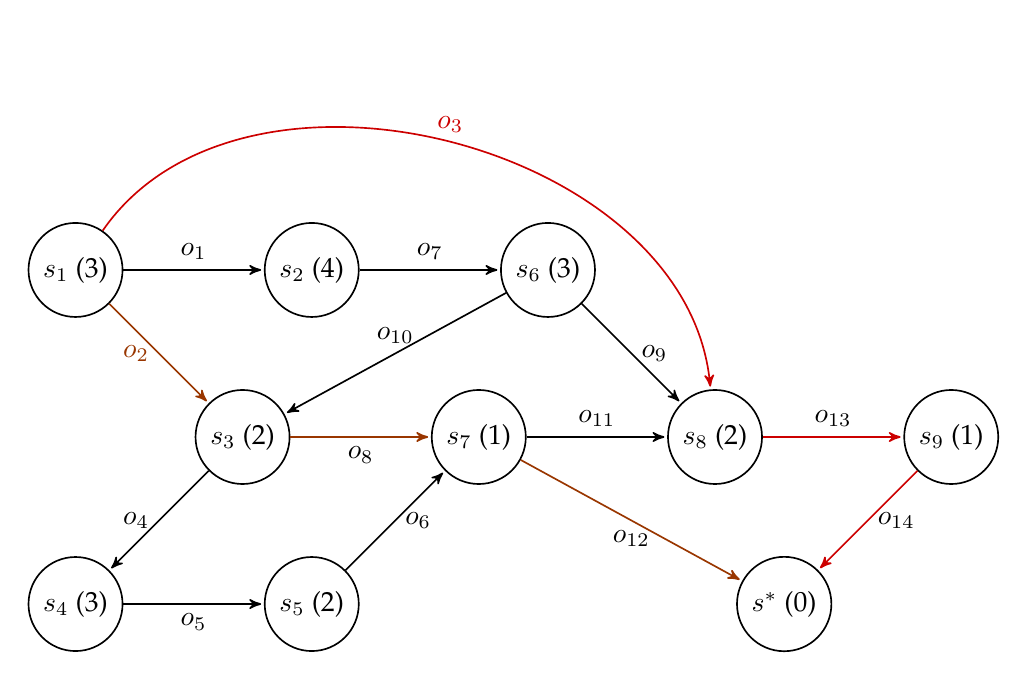
\begin{tikzpicture}[->,>=stealth',shorten >=1pt,auto,node distance=3cm,semithick]
  \tikzstyle{state}=[circle,draw,minimum size=1cm]

  \node[state] (s1) {$s_1$ (3)};
  \node[state] (s2) [right of=s1] {$s_2$ (4)};
  \node[state] (s3) [below right of=s1] {$s_3$ (2)};
  \node[state] (s4) [below left of=s3] {$s_4$ (3)};
  \node[state] (s5) [right of=s4] {$s_5$ (2)};
  \node[state] (s6) [right of=s2] {$s_6$ (3)};
  \node[state] (s7) [right of=s3] {$s_7$ (1)};
  \node[state] (s8) [below right of=s6] {$s_8$ (2)};
  \node[state] (s9) [right of=s8] {$s_9$ (1)};
  \node[state] (s10) [below left of=s9] {$s^*$ (0)};

  \path (s1) edge node[above] {$o_{1}$} (s2);
  \path [->, color=myorange] (s1) edge node[left] {$o_{2}$} (s3);
  \path [->, color=myred] (s1) edge [bend left=70] node[above] {$o_{3}$} (s8);
  \path (s2) edge node[above] {$o_{7}$} (s6);
  \path (s3) edge [draw=myorange] node[below] {$o_{8}$} (s7);
  \path (s3) edge node[left] {$o_{4}$} (s4);
  \path (s4) edge node[below] {$o_{5}$} (s5);
  \path (s5) edge node[right] {$o_{6}$} (s7);
  \path (s6) edge node[right] {$o_{9}$} (s8);
  \path (s6) edge node[above] {$o_{10}$} (s3);
  \path (s7) edge node[above] {$o_{11}$} (s8);
  \path (s7) edge [draw=myorange] node[below] {$o_{12}$} (s10);
  \path (s8) edge [draw=myred] node[above] {$o_{13}$} (s9);
  \path (s9) edge [draw=myred] node[right] {$o_{14}$} (s10);
\end{tikzpicture}
\label{fig:spg-example}
\end{figure}


\section{Generating Samples with \bfsrs}
\label{sec:sample-learn-po}
The sample generation approach described in~\cref{sec:sample-learn-h} is unsuitable for learning preferred operators due to duplicate samples within rollouts. This leads to a sample set that contains numerous repeated samples, which offer no additional value when constructing the shortest path graph $G'$ for identifying preferred operators. Consequently, this approach fails to expand the state space and identify additional preferred operators effectively. To address this, we developed a new sample generation method designed to discover preferred operators, dubbed ``expansion from random successors''~(\bfsrs), divided into two phases.

Let $S_1$ and $S_2$ denote the sets of samples generated in the first and second phases of~\bfsrs. The complete sample set is represented by $S = S_1 \cup S_2$, consisting of $N$ distinct samples. Let $k_1$ and $k_2$ be variables satisfying $k_1 + k_{2} = 1$.
In the first phase of the algorithm, we use BFS by applying backward applicable operators from the goal condition until expanding $k_1N$ states, which are then added to $S_1$.
In the second phase, we maintain two structures first initialized during BFS: an open queue, containing states generated but not yet expanded, and a closed set, comprising states that have been expanded and already sampled. During each iteration, we randomly select a state from the open queue, move it to the closed set, add it to the sample set $S_2$, and insert its predecessors into the open queue if they are not already present in open or closed. The sampling process continues until $|S_2| = k_2N$.
See \cref{alg:sampling-po}. The primary distinction between phases one and two is the selection process for expanding states from the open queue. Unlike phase one, where the first-in, first-out approach of BFS is used, phase two involves randomly selecting a state from the open queue for expansion. We do not use a regression limit $L$ as in \bfsrw, but in practice our maximum regression depth remained close to $d^{*}$~(\vref{cha:max_reg_depth}).

\begin{algorithm}[tb]
\caption{Sampling states using \bfsrs}
\label{alg:sampling-po}
\begin{algorithmic}[1]
\Procedure{\bfsrs}{$s^{*}$, $N$, $k_{1}$, $k_{2}$}
  \State $open = \emptyset$
  \State $S_{1} = \emptyset$
  \State \textcolor{gray}{\# Phase 1: populates $S_{1}$ and $open$ with BFS.}
  \State $S_{1}, open \gets$ BFS($s^{*}$, $open$, $k_1N$)
  \State $closed = S_{1}$
  \State \textcolor{gray}{\# Phase 2: populates $S_{2}$ with random elements $s$ from $open$.}
  \State $S_{2} = \emptyset$
  \While{$|S_{2}| < k_{2}N$}
    \If{$open =  \emptyset$}
      \State \textbf{return} $S_{1} \cup S_{2}$ (backward state space fully expanded)
    \EndIf

    \State $i \gets$ random index of $open$
    \State \textcolor{gray}{\# Initialize a partial state $s$.}
    \State $s \gets$ $open$[$i$]
    \State Remove element at $open$[$i$]
    \State $closed \gets closed \cup \{s\}$
    \State $S_{2} \gets S_{2} \cup \{s\}$
    \State $P \gets \{s' \mid s' \in pred(s)\}$
    \ForAll{partial states $s' \in P$}
      \If{$s' \notin (open \cup closed)$}
        \State Insert $s'$ into $open$
      \EndIf
    \EndFor
  \EndWhile

  \State \textbf{return} $S_{1} \cup S_{2}$
\EndProcedure
\end{algorithmic}
\end{algorithm}

%\begin{algorithm}[tb]
%\caption{Breadth-first search of \bfsrs}
%\label{alg:sampling-bfs}
%\begin{algorithmic}[1]
%\Procedure{BFS}{$s^{*}$, $open$, $M$}
%  \State $S_{1} = \emptyset$
%  \State $open \gets open \cup \{s^{*}\}$
%
%  \While{$|S_{1}| < M$}
%    \If{$open =  \emptyset$}
%      \State \textbf{return} $S_{1}$ (backward state space fully explored)
%    \EndIf
%    \State \textcolor{gray}{\# Initialize a partial state $s$}
%    \State $s \gets$ first element in $open$
%    \State Remove first element in $open$
%    \State $S_{1} \gets S_{1} \cup \{s\}$
%    \State $P \gets \{s' \mid s' \in pred_{bfs}(s)\}$
%    \ForAll{partial state $s' \in P$}
%      \If{$s' \notin open$}
%        \State $open \gets open \cup \{s'\}$
%      \EndIf
%    \EndFor
%  \EndWhile
%
%  \State \textbf{return} $S_{1}$
%\EndProcedure
%\end{algorithmic}
%\end{algorithm}

After regression, we apply \sai and \sui and complete the states as described in~\cref{sec:sample-improving-h,sec:sample-completion}. We compare \bfsrs with \bfsrw for discovering preferred operators in~\cref{sec:exp-comparison-sample-method}.

%\section{Randomly Generated Samples}
%\label{sec:sample-random-samples}
%\citet{OToole/2022} demonstrated that augmenting a sample set generated through expansion with randomly generated samples enhances the performance of the search algorithm guided by the learned heuristic. They suggest assigning a cost-to-goal estimate of $L+1$ to randomly generated samples, where $L$ represents the maximum regression limit.
%The samples are generated from undefined states and are completed as discussed in~\cref{sec:sample-completion}. If the generated state $s$ is already present in the sample set, denoted as $s = s_i$ for some $i\in[N]$, it is assigned the cost-to-goal estimate $h_i$. Conversely, if the state $s$ is not already in the sample set, it is given a cost-to-goal estimate of $1+\max_{i\in[N]} h_i$, ensuring that the estimate is larger than all existing estimates.

%
% - - - - - - - - - - - - - - - -- - - - - -
% experiments
% - - - - - - - - - - - - - - - -- - - - - -
% empiricism!
%
\chapter{Experiments}
\label{cha:exp-experiments}
This section presents four experiments. In the first (\cref{sec:exp-learning-po}), we investigate learning preferred operators and establish an upper-bound performance measure using the ideal preferred operators, comparing them to the proposed approach. The second experiment (\cref{sec:exp-performance-po}) evaluates learning discovered preferred operators from sample sets of varying sizes and compares them to a logic-based preferred operator. The third experiment (\cref{sec:exp-comparison-sample-method}) compares the results with preferred operators learned from a sample set generated using two distinct sampling methods, as described in~\cref{sec:sample-learn-h} and~\cref{sec:sample-learn-po}. Finally, in the fourth experiment~(\cref{sec:other-heuristic-functions}), we analyze the learned preferred operators in conjunction with several logic-based heuristic functions.


\section{Configuration}
\label{sec:exp-configuration}

We use the same network architecture as \citet{Ferber.etal/2022},~\citet{OToole/2022}, and~\citet{Bettker.etal/2022} with modifications to support learning preferred operators. Specifically, we use a ResNet with He initialization~\cite{He.etal/2015}, consisting of two hidden layers followed by a residual block containing two hidden layers.
Each hidden layer has $250$ neurons and is ReLU-activated.
The training uses the Adam optimizer~\cite{Kingma.Ba/2015} with a learning rate of $10^{-4}$, a batch size of $64$, and a patience of $100$ epochs.
We use the MSE loss function to learn heuristic values in a regression context, and for learning preferred operators, we opt for the BCE loss since learning preferred operators is a multi-label classification problem.
The input of the NN consists of samples in the format $(h(s), \mathcal{F}(s), O_{pref} \subseteq O)$
where $\mathcal{F}(s)$ is a Boolean representation of the input state $s$, with $0$ if a proposition is false and $1$ otherwise~(\cref{sec:background-heuristics}), $h(s)$ is the target value in the regression network representing the $h$-value for $s$, and $O_{pref}$ are the target values in the classification network representing the preferred operators for state $s$.

The output for the regression network is a single ReLU-activated neuron representing the learned $h$-value, and the output for classification is a sigmoid-activated tensor with values in the range $[0, 1]$ and a size equal to the number of operators of the input task.
In the case of classification, each output neuron corresponds to an indexed operator. For example, in a planning task with ten operators, in which a sampled state $s$ has target preferred operators two and five, the indexes two and five of the output tensor must be maximized~(\cref{fig:po-tensor}). Finally, the training set has $90\,\%$ of the data, while the validation set contains the remaining $10\,\%$.

\begin{figure}[tb]
\caption[]{Example tensor with two preferred operators as target values.}
\vspace{\baselineskip}
\centering
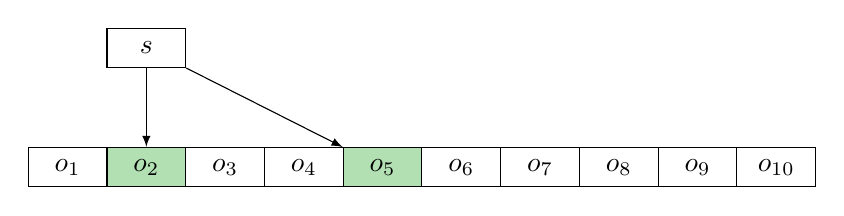
\begin{tikzpicture}[node distance=1cm]
  % Operators
  %\foreach \x in {1,...,10}
  %  \node[draw, minimum width=1cm, minimum height=0.5cm] (op\x) at (\x,0) {$o_{\x}$};
  \foreach \x in {1,...,10}{
    \ifnum\x=2
      \node[draw, minimum width=1cm, minimum height=0.5cm, fill=mygreen!30] (op\x) at (\x,0) {$o_{\x}$};
    \else
      \ifnum\x=5
        \node[draw, minimum width=1cm, minimum height=0.5cm, fill=mygreen!30] (op\x) at (\x,0) {$o_{\x}$};
      \else
        \node[draw, minimum width=1cm, minimum height=0.5cm] (op\x) at (\x,0) {$o_{\x}$};
      \fi
    \fi
  }
  % Sampled state
  \node[draw, minimum width=1cm, minimum height=0.5cm, above=of op2] (s) {$s$};

  % Arrows
  \draw[->] (s) -- (op2);
  \draw[->] (s) -- (op5);
\end{tikzpicture}
\label{fig:po-tensor}
\end{figure}


\subsection{Extracting Preferred Operators}
\label{sec:exp-extracting-pos}
We extract the predicted preferred operators from the NN by selecting the operator with the highest output value. Additionally, if there are any operators with output values greater than $0.9$, we include them in the selection. We do this to avoid false positives since most tasks considered in this work have a mean number of preferred operators close to one. Through experimentation, we found that this strategy produced better results than selecting only operators with output values above an arbitrary threshold, as lowering the threshold resulted in poorer performance.


\subsection{Dataset}
\label{sec:exp-dataset}
Our dataset consists of planning tasks with unitary operators and state spaces ranging from $40$\,K to $1$\,M states, identical to the dataset used by~\citet{Bettker.etal/2022}. To generate samples, we use one task in each of the following domains: Blocks World (abbreviated as Blocks), Grid, N-Puzzle, Rovers, Scanalyzer, Transport, and VisitAll. \cref{tab:tasks_info} has relevant information regarding each task, and~\vref{cha:tasks_each_domain} contains a small description of each domain. The output neurons in the classification NN correspond to the number of operators, whereas the regression NN used for learning heuristics produces a single numerical value as its output. The number of facts determines the input neurons.

We evaluate the results based on the number of expanded states since all planning tasks are solved. Each forward state space \fsp has $50$ randomly generated initial states, resulting in $50$ planning tasks. %We generate these initial states by conducting a random walk of length $200$ from the original initial state of a task. However, in the Rovers, Scanalyzer, and VisitAll domains, some initial states were duplicated or already satisfied the goal condition. As a result, we generate initial states for these domains using random walks of length $25$, $50$, and $8$, respectively.
In the tables, each cell represents the mean value across $50$ planning tasks and $25$ seeds, i.e., $5$ sample seeds $\times$ $5$ network seeds. Each sample seed represents a different set of samples, while the network seeds are used to initialize the parameters of the NN.
Additionally, when referring to a specific number of samples, we use the notation ``$n$ percent of the state space'' to denote a fraction of the \fsp, e.g., $5\,\%$ of Block World's \fsp is $\lfloor 65990 \times 0.05 \rceil = 3300$ samples.

\begin{table}[htb]
\centering
\caption{Information on the task used for each domain. The forward state space size, the distance \distfarthest of the state most distant from the goal state, regression limit $L$, the number of facts, and the number of operators.}
\vspace{\baselineskip}
\begin{tabular}{lrrrrr}
\toprule
Domain     & FSS size & \distfarthest & $L$  & \# facts & \# operators \\ \midrule
Blocks     & 65990    & 24            & 17   & 64       & 98           \\
Grid       & 452353   & 32            & 44   & 76       & 252          \\
N-Puzzle   & 181440   & 31            & 41   & 81       & 192          \\
Rovers     & 565824   & 19            & 27   & 32       & 57           \\
Scanalyzer & 46080    & 15            & 20   & 42       & 300          \\
Transport  & 637632   & 17            & 35   & 66       & 572          \\
VisitAll   & 79931    & 15            & 17   & 31       & 48           \\ \bottomrule
\end{tabular}
\label{tab:tasks_info}
\end{table}



\subsection{Training}
\label{sec:exp-training}
We implement sample generation in Neural Fast Downward~\cite{Ferber.etal/2020a} and use PyTorch 1.9.0~\cite{Paszke/2019} to define and train the NNs. We conducted the experiments on Ubuntu~$20.04$~LTS~GNU/Linux machines with an AMD~Ryzen~$9$~$3900$X $12$-core processor ($4.2$~GHz), a memory limit of $4$~GB, and one core per process. The NNs were trained until convergence, with the most complex networks requiring approximately two hours of training~(\vref{cha:training_details}).%\footnote{Source code available at \url{https://github.com/pprobst/NeuralFastDownward}.}

\subsection{Evaluation}
\label{sec:exp-evaluation}
We measure search performance by the number of expanded states since we have perfect coverage for all the selected domains. We use the Fast Downward planning system~\cite{Helmert/2006} with GBFS guided by a heuristic function to solve all $50$ initial states of each domain using a $5$ minute search time limit for each initial state.
When preferred operators are used along the heuristic function, we experimented with searches using dual-queues with and without boosting. Due to better experimental results, for the following experiments, we use a boosted dual-queue with a boost value of $1000$, as in~\citet{Richter.Helmert/2009}. Results for searches with boosting disabled are available in~\vref{cha:discovered_pos_boost0}.

\subsection{Sampling}
\label{sec:exp-sampling}
We obtain the learned heuristic \hnn by training over samples generated as described in~\cref{sec:sample-learn-h}, with the best configuration from~\citet{Bettker.etal/2022}, i.e., sample set size equal to $1\,\%$ of the state space, regression limit of $L=\ceil{\facts/\overline{\eff}}$, and setting the quantity of samples generated by BFS to $p_{\bfsrw}=10\,\%$ of the total number of samples. As~\citet{Bettker.etal/2022}, $20\,\%$ of the total number of samples are randomly generated samples, with cost-to-goal estimates equal to the maximum estimate of the existing samples obtained through regression plus one.

Since in this work we are only interested in the effects of learned preferred operators, the learned heuristic functions \hnn for each task have the fixed configuration described earlier. To obtain the learned discovered preferred operators \pog, we train the NNs over sample sets generated according to the method described in~\cref{sec:sample-learn-po}, with $k_1 = 0.1$ and $k_2 = 0.9$, since these values had better results in preliminary experiments (\vref{cha:bfsss_pct}). In this configuration, we do not use randomly generated samples.


\section{Learning Preferred Operators}
\label{sec:exp-learning-po}
This section establishes baselines for comparing our proposed approach of learned discovered operators. In particular, we compare task-solving performance with several configurations. We present results using GBFS guided by the perfect heuristic \hstar and the learned heuristic \hnn, with and without preferred operators. We also use two classes of preferred operators. The first class represents the ideal preferred operators \postartable and \postar, where \postartable is an oracle and \postar was trained over the complete \fsp of each task. The second class represents the proposed approach with learned discovered operators \pogstar and \pog, which were trained on a $1\,\%$ sample set obtained through regression with the method described in~\cref{sec:sample-learn-po}, the only difference being that \pogstar has perfect \hstar-values for each sample.

\begin{table}[tb]
\centering
\caption[Expansions of \hstar, \hnn, \postartable, \postar, \pogstar, and \pog]{Expanded states for various approaches using GBFS. The ``Baseline'' approach refers to searches using only the optimal heuristic \hstar and the learned heuristic \hnn. The ``Ideal'' approach represents searches using \hnn with ideal preferred operators, while the ``$G'$'' approach is \hnn with shortest-path-graph-based preferred operators.}
\label{tab:learning_perfect_pos}
\vspace{\baselineskip}
\begin{tabular}{lrrrrrr}
\toprule
           & \multicolumn{2}{c}{Baseline} & \multicolumn{2}{c}{Ideal} & \multicolumn{2}{c}{$G'$} \\
           \cmidrule(lr){2-3}\cmidrule(lr){4-5}\cmidrule(lr){6-7}
Domain     & \hstar & \hnn & \postartable & \postar & \pogstar & \pog \\ \midrule
Blocks     & 19.4   & 57.0 & 21.0          & 42.1     & 43.0   & 43.0  \\
Grid       & 20.8   & 66.5 & 23.1          & 23.2     & 70.4   & 67.4  \\
N-Puzzle   & 22.6   & 80.9 & 23.9          & 28.0     & 53.3   & 53.3  \\
Rovers     & 10.3   & 13.4 & 10.7          & 10.6     & 12.2   & 12.2  \\
Scanalyzer & 9.2    & 28.3 & 10.6          & 10.7     & 29.1   & 30.7  \\
Transport  & 13.3   & 25.2 & 13.9          & 13.9     & 21.3   & 21.4  \\
VisitAll   & 11.9   & 21.8 & 12.8          & 12.8     & 21.2   & 20.5  \\ \midrule
Geo. mean  & 14.5   & 35.0 & 15.7          & 17.7     & 30.7   & 30.6  \\ \bottomrule
\end{tabular}
\end{table}


\cref{tab:learning_perfect_pos} shows that all approaches using preferred operators lead to fewer expansions than using only the learned heuristic \hnn. In particular, \hnn with the ideal preferred operators \postartable and \postar closely approach the optimal expansion values with \hstar.
The ideal preferred operators serve as performance limits, representing the best achievable results as defined in \cref{sec:sample-ideal-po}. When comparing the learned ideal preferred operators \postar with the oracle \postartable, we find that the NN can learn the preferred operators for the entire state space in all domains, except for Blocks World and N-Puzzle, where performance degrades but remains better than \hnn.

The learned ideal preferred operators~\postar surpass using only the learned heuristic \hnn in all domains. They significantly reduce the number of expansions by over $50\,\%$ in Grid, N-Puzzle, and Scanalyzer. When we reduce the state space to $1\,\%$ and use the shortest path graph $G'$ to identify preferred operators, the proposed approach~\pog exhibits an increase of approximately $73\,\%$ in the geometric mean of expanded states compared to the learned ideal preferred operators \postar. Still, \hnn with \pog expand fewer states than using only \hnn in all domains except Grid and Scanalyzer, with significant improvements in mean expansions of approximately $25\,\%$ and $34\,\%$ observed in Blocks World and N-Puzzle, respectively.

%The effectiveness of preferred operators may inversely correlate with the quality of the heuristic function. When the heuristic function is nearly optimal, the inclusion of preferred operators can potentially interfere with the search process. In \cref{sec:other-heuristic-functions}, we explore the outcomes observed when using different logic-based heuristics with varying levels of quality.

When comparing the discovered preferred operators \pogstar to \pog, both have close results despite \pogstar using the perfect heuristic \hstar to calculate the shortest paths in the sample set. The reason for this similarity is that the arcs in the shortest path graph $G'$ for \pog are largely retained when compared to \pogstar, and equivalent states in the sample sets of both methods tend to have similar preferred operators, indicating that they are likely to have similar shortest paths to follow. In particular, close to $100\,\%$ of the samples have the same set of preferred operators in \pogstar and \pog in all domains except Scanalyzer ($92\,\%$) and VisitAll ($68\,\%$). For all states with different preferred operators in all domains, the preferred operators of \pog are a subset of the preferred operators of \pogstar. As seen in \cref{tab:learning_perfect_pos}, this difference is negligible for Scanalyzer and VisitAll, where \pogstar and \pog differ by less than one expansion on average. This result indicates that discovering preferred operators from the shortest path graph $G'$ with quality similar to ideal preferred operators is possible even without perfect \hstar-values.

This experiment demonstrated the effectiveness of learning high-quality preferred operators that enhance suboptimal heuristics. The learned ideal preferred operators \postar outperformed \hnn in all domains, improving the geometric mean of expansions by about $50\,\%$. The proposed approach \pog had fewer expansions than \hnn in five out of seven domains, improving the geometric mean by approximately $13\,\%$.


\section{Discovering Preferred Operators on Different Sample Set Sizes}
\label{sec:exp-performance-po}
In this experiment, we use GBFS guided by the learned heuristic \hnn and compare the learned discovered preferred operators \pog to the logic-based preferred operators \poff from FF~\cite{Hoffmann.Nebel/2001} implemented in Fast Downward~\cite{Helmert/2006}. In addition to using a sample set equivalent to $1\,\%$ of the forward state space, as in the previous experiment, we also examine other percentages: $5,\%$, $10\,\%$, $20\,\%$, $30\,\%$, $40,\%$, $50\,\%$. \cref{tab:learning_discovered_pos} shows the results.

\begin{table}[tb]
\centering
\caption[Expansions of \hnn, \poff, and \pog]{Number of expansions of \hnn with no preferred operators, with \poff and with \pog trained with the discovered learned operators with varying the size of the sample set according to different percentages of the state space size. Rovers maintained the same results from $20\,\%$ onwards as they sampled the complete backward state space, which numerically represents approximately $15\,\%$ of the forward state space. }
\label{tab:learning_discovered_pos}
\vspace{\baselineskip}
\begin{tabular}{lrrrrrrrrr}
\toprule
           &     &        & \multicolumn{7}{c}{$\pog$} \\
\cmidrule(lr){4-10}
Domain     & \hnn & \poff & $1$ & $5$   & $10$ & $20$ & $30$ & $40$ & $50$ \\ \midrule
Blocks     & 57.0 & 41.1  & 43.0 & 26.2 & 29.6 & 32.2 & 34.9 & 38.0 & 38.8 \\
Grid       & 66.5 & 32.7  & 67.4 & 53.0 & 46.4 & 27.4 & 23.8 & 23.6 & 22.9 \\
N-Puzzle   & 80.9 & 100.2 & 53.3 & 34.8 & 31.6 & 28.5 & 28.1 & 27.4 & 27.4 \\
Rovers     & 13.4 & 18.5  & 12.2 & 11.7 & 13.0 & 17.2 & 17.2 & 17.2 & 17.2 \\
Scanalyzer & 28.3 & 17.1  & 30.7 & 18.1 & 13.0 & 11.7 & 11.5 & 11.6 & 11.5 \\
Transport  & 25.2 & 17.0  & 21.4 & 16.3 & 15.8 & 15.1 & 14.7 & 14.4 & 14.3 \\
VisitAll   & 21.8 & 18.7  & 20.5 & 17.1 & 15.7 & 15.7 & 15.8 & 16.1 & 16.3 \\ \midrule
Geo. mean  & 35.0 & 28.0  & 30.6 & 22.4 & 21.0 & 19.8 & 19.5 & 19.7 & 19.6 \\ \bottomrule
\end{tabular}
\end{table}


By increasing the sample set size, the number of arcs and vertices in the shortest path graph $G'$ expands, leading to the discovery of new shortest paths. As expected, the performance of the learned discovered preferred operators \pog improves as the sample set size increases, reaching a plateau after $20\,\%$. However, Rovers shows an exception where the learned preferred operators result in increased expansions after $5\,\%$. In this domain, both the logic-based preferred operators \poff and \pog trained on a $1\,\%$ sample set size yield worse results than \hnn alone. This suggests that in Rovers, preferred operators may not be helpful since \hnn already approaches optimality ($13.4$ vs. $10.3$), as shown in~\cref{tab:learning_perfect_pos}.

As shown in~\cref{sec:background-preferred-operators}, in Fast Downward, repeated generated states are not added to the preferred queue. This is more significant in Blocks World and Rovers, increasing the number of expansions. Furthermore, this happens more frequently when training over larger sample sets, as multiple preferred operators are predicted more frequently. To mitigate this issue, a potential approach may be disabling boosting or using a more restrictive threshold when extracting preferred operators.
% To address this, we can select only the preferred operator with the highest output value from the NN. With this approach, Blocks World and Rovers stabilize from $10\,\%$ onward at approximately $27$ and $12$ expansions, respectively, while the other domains do not experience significant changes.

Training with $5\,\%$ of the sample set size is sufficient to achieve $20\,\%$ fewer expansions on average compared to~\poff, i.e., the learned preferred operators \pog can outperform logic-based ones given a large enough sample set size. Specifically, with $5\,\%$, we achieve better results than \poff except in Grid ($53.0$ vs. $32.7$) and Scanalyzer ($18.1$ vs. $17.1$). However, as the sample size increases, we eventually surpass \poff in all domains. Moreover, the use of logic-based preferred operators \poff leads to degraded performance in N-Puzzle compared to only using \hnn, while \pog with a $1\,\%$ sample set substantially improves it.

\cref{fig:errors} shows the standard deviations for the expansions in~\cref{tab:learning_discovered_pos}. Smaller sample sets generally exhibit higher variability in the number of expanded states. For instance, with a $1\,\%$ sample set size, Blocks World, Grid, N-Puzzle, and Scanalyzer have standard deviations of approximately $12$, $27$, $8$, and $10$, respectively. As the sample set size increases, the standard deviation decreases, except for Blocks World, which maintains a standard deviation of approximately $10$. Notably, all domains, except Blocks World, have standard deviation values close to one for sample set sizes of $20\,\%$ and above. \citet{Bettker.etal/2022} also observed similar variability in their results.

\begin{figure}[tb]
  \caption[Standard deviation of expansions using \hnn with \pog]{Mean number of expansions and its standard deviation per domain for GBFS guided by \hnn with \pog trained using sample sets of different sizes.}
  \centering
  \vspace{\baselineskip}
  \begin{subfigure}{0.41\textwidth}
    \centering
    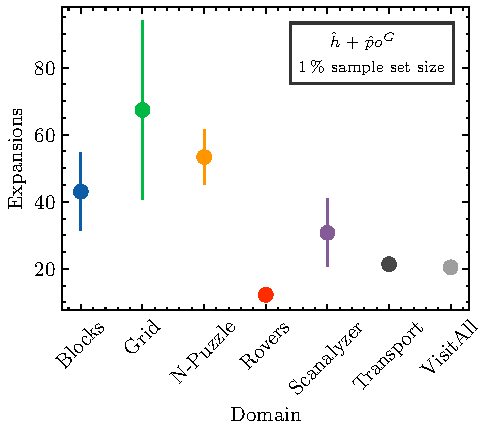
\includegraphics[width=\linewidth]{img/error_hNN_poG_1pct.pdf}
  \end{subfigure}
  %\hfill
  \begin{subfigure}{0.41\textwidth}
    \centering
    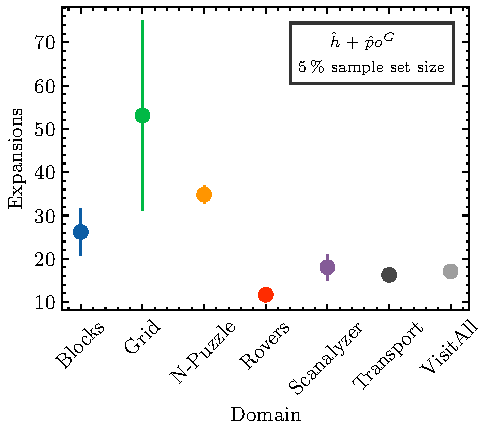
\includegraphics[width=\linewidth]{img/error_hNN_poG_5pct.pdf}
  \end{subfigure}


  \vspace{0.5cm}

  %\hfill
  \begin{subfigure}{0.41\textwidth}
    \centering
    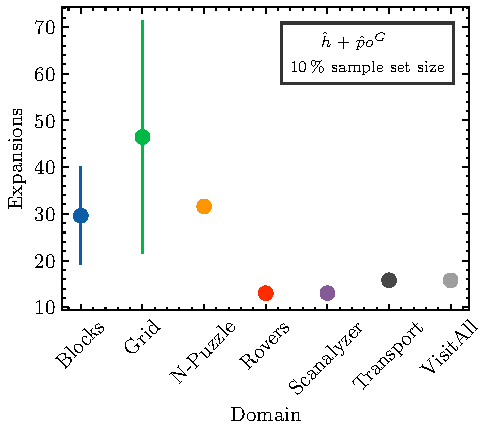
\includegraphics[width=\linewidth]{img/error_hNN_poG_10pct.pdf}
  \end{subfigure}
  \begin{subfigure}{0.41\textwidth}
    \centering
    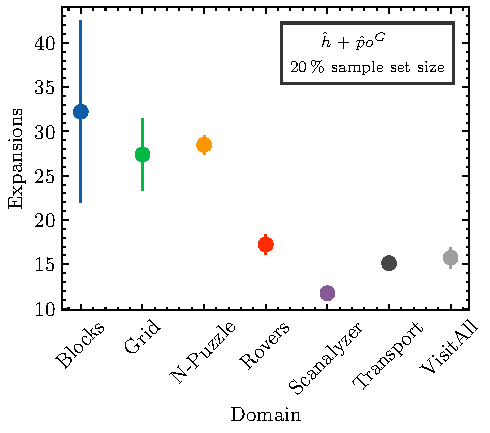
\includegraphics[width=\linewidth]{img/error_hNN_poG_20pct.pdf}
  \end{subfigure}
  %\hfill

  \vspace{0.5cm}

  \begin{subfigure}{0.41\textwidth}
    \centering
    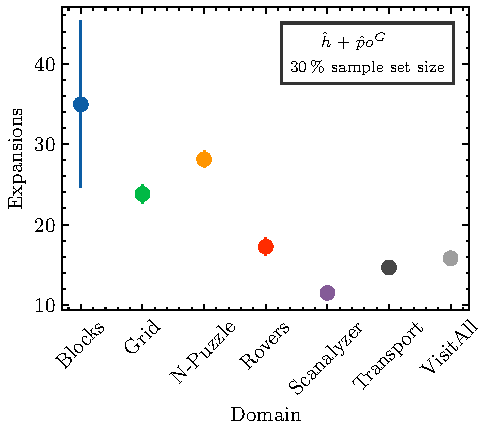
\includegraphics[width=\linewidth]{img/error_hNN_poG_30pct.pdf}
  \end{subfigure}
  %\hfill
  \begin{subfigure}{0.41\textwidth}
    \centering
    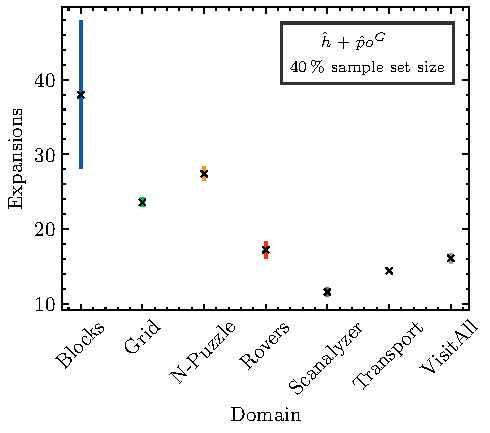
\includegraphics[width=\linewidth]{img/error_hNN_poG_40pct.pdf}
  \end{subfigure}

  \vspace{0.5cm}

  \begin{subfigure}{0.41\textwidth}
    \centering
    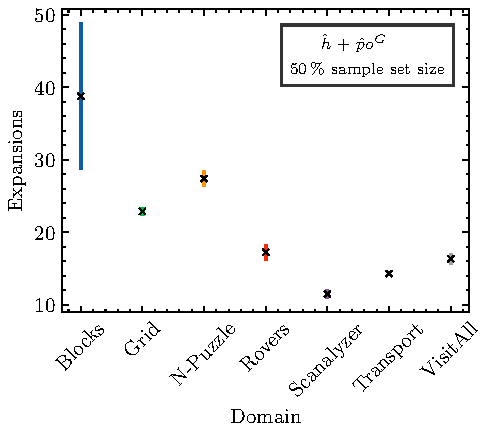
\includegraphics[width=\linewidth]{img/error_hNN_poG_50pct.pdf}
  \end{subfigure}
  \label{fig:errors}
\end{figure}


\section{Comparison to Alternative Sampling Method}
\label{sec:exp-comparison-sample-method}
This experiment compares the number of expansions between two methods for discovering operators. The first method is the sampling approach proposed in \cref{sec:sample-learn-po}, while the second method is the one introduced by~\citet{Bettker.etal/2022} and described in \cref{sec:sample-learn-h} (differently from learning \hnn, we exclude randomly generated samples since applicable operators do not necessarily generate them). \cref{tab:comparison_sample} shows the results.

The learned preferred operators \pog consistently expands fewer states than \pofsm, except for Blocks World (from $20\,\%$ onward) and VisitAll. Considering all the sample set sizes, \pog has about $14\,\%$ fewer expansions on average. Notably, \pofsm needs ten times the number of samples (e.g., $50\,\%$ vs. $5\,\%$) to achieve comparable results to \pog on average, highlighting the efficiency of \bfsrs in contrast to \bfsrw when it comes to learning preferred operators.

In~\cref{sec:sample-learn-po} we mention~\bfsrw has many repeated states, which are not considered when constructing the shortest path graph. To provide quantitative insights, we examined a sample set size of $5\,\%$ consisting of samples with partial states (without completion). While $100\,\%$ of the states generated by \bfsrs in all domains are unique, for \bfsrw the percentages of unique states are as follows: $72\,\%$ in Blocks World, $84\,\%$ in Grid, $96\,\%$ in N-Puzzle, $58\,\%$ in Rovers, $89\,\%$ in Scanalyzer, $96\,\%$ in Transport, and $86\,\%$ in VisitAll.

\begin{table}[tb]
\centering
%\small
%\setlength{\tabcolsep}{0.9ex}
\caption[Expansions of \pog and \pofsm]{Expansions of GBFS guided by \hnn with \pog and \pofsm using FSM from~\citet{Bettker.etal/2022}, varying the size of the sample set according to different percentages of the forward state space size.}
\label{tab:comparison_sample}
\vspace{\baselineskip}
\begin{tabular}{lrrrrrrrrrr}
\toprule
           &  \multicolumn{2}{c}{$1\,\%$} & \multicolumn{2}{c}{$5\,\%$} & \multicolumn{2}{c}{$10\,\%$} & \multicolumn{2}{c}{$20\,\%$} \\
\cmidrule(lr){2-3} \cmidrule(lr){4-5} \cmidrule(lr){6-7} \cmidrule(lr){8-9}
Domain     &  \pog  & \pofsm & \pog  & \pofsm & \pog & \pofsm & \pog & \pofsm \\ \midrule
Blocks     &  \textbf{43.0}  & 56.8   & \textbf{26.2}  & 31.7 & \textbf{29.6} & 30.4 & \textbf{32.2} & 32.8    \\
Grid       &  \textbf{67.4}  & 74.3   & \textbf{53.0}  & 67.8 & \textbf{46.4} & 67.3 & \textbf{27.4} & 69.9    \\
N-Puzzle   &  \textbf{53.3}  & 67.6   & \textbf{34.8}  & 48.5 & \textbf{31.6} & 38.1 & \textbf{28.5} & 32.3   \\
Rovers     &  12.2  & \textbf{12.1}   & \textbf{11.7}  & 13.1 & \textbf{13.0} & 15.7 & \textbf{17.2} & 19.9   \\
Scanalyzer &  \textbf{30.7}  & 33.7   & \textbf{18.1}  & 21.0 & \textbf{13.0} & 14.5 & \textbf{11.7} & 11.9   \\
Transport  &  \textbf{21.4}  & 23.6   & \textbf{16.3}  & 19.9 & \textbf{15.8} & 18.2 & \textbf{15.1} & 16.9   \\
VisitAll   &  20.5  & \textbf{19.8}   & 17.1  & \textbf{15.6} & 15.7 & \textbf{15.3} & 15.7 & \textbf{14.8}   \\ \midrule
Geo. mean  &  \textbf{30.6}  & 34.2   & \textbf{22.4}  & 26.4 & \textbf{21.0} & 24.3 & \textbf{19.8} & 23.8  \\ \midrule
\end{tabular}

\begin{tabular}{lrrrrrrrrrrrr}
           &  \multicolumn{2}{c}{$30\,\%$} & \multicolumn{2}{c}{$40\,\%$} & \multicolumn{2}{c}{$50\,\%$} &&&&&& \\
\cmidrule(lr){2-3} \cmidrule(lr){4-5} \cmidrule(lr){6-7}
     &   \pog & \pofsm & \pog & \pofsm & \pog & \pofsm &&&&&& \\ \midrule
Blocks     &  34.9 & \textbf{33.2} & 38.0 & \textbf{32.1} & 38.8 & \textbf{32.3} &&&&&& \\
Grid       &  \textbf{23.8} & 64.5 & \textbf{23.6} & 59.1 & \textbf{22.9} & 55.0 &&&&&& \\
N-Puzzle   &  \textbf{28.1} & 29.6 & \textbf{27.4} & 28.9 & \textbf{27.4} & 27.7 &&&&&& \\
Rovers     &  \textbf{17.2} & 20.8 & \textbf{17.2} & 21.3 & \textbf{17.2} & 21.4 &&&&&& \\
Scanalyzer &  \textbf{11.5} & 11.6 & 11.6 & \textbf{11.5} & \textbf{11.5} & 11.7 &&&&&& \\
Transport  &  \textbf{14.7} & 16.1 & \textbf{14.4} & 15.8 & \textbf{14.3} & 15.5 &&&&&& \\
VisitAll   &  15.8 & \textbf{14.9} & 16.1 & \textbf{15.6} & 16.3 & \textbf{15.4} &&&&&& \\ \midrule
Geo. mean  &  \textbf{19.5} & 23.2 & \textbf{19.7} & 22.9 & \textbf{19.6} & 22.5 &&&&&& \\ \bottomrule
\end{tabular}
\end{table}

\iffalse
\begin{table}[!h]
\centering
\small
\setlength{\tabcolsep}{0.9ex}
\caption{Number of expansions GBFS guided by \hnn with \pog and \pofsm, varying the size of the sample set according to different percentages of the state space size.}
\label{tab:comparison_sample}
\vspace{\baselineskip}
\begin{tabular}{lrrrrrrrrrrrrrr}
\toprule
           &  \multicolumn{2}{c}{$1$} & \multicolumn{2}{c}{$5$} & \multicolumn{2}{c}{$10$} & \multicolumn{2}{c}{$20$} & \multicolumn{2}{c}{$30$} & \multicolumn{2}{c}{$40$} & \multicolumn{2}{c}{$50$} \\
\cmidrule(lr){2-3} \cmidrule(lr){4-5} \cmidrule(lr){6-7} \cmidrule(lr){8-9} \cmidrule(lr){10-11} \cmidrule(lr){12-13} \cmidrule(lr){14-15}
Domain     &  \pog  & \pofsm & \pog  & \pofsm & \pog & \pofsm & \pog & \pofsm & \pog & \pofsm & \pog & \pofsm & \pog & \pofsm \\ \midrule
Blocks     &  43.0  & 56.8   & 26.2  & 31.7 & 29.6 & 30.4 & 32.2 & 32.8 & 34.9 & 33.2 & 38.0 & 32.1 & 38.8 & 32.3 \\
Grid       &  67.4  & 74.3   & 53.0  & 67.8 & 46.4 & 67.3 & 27.4 & 69.9 & 23.8 & 64.5 & 23.6 & 59.1 & 22.9 & 55.0 \\
N-Puzzle   &  53.3  & 67.6   & 34.8  & 48.5 & 31.6 & 38.1 & 28.5 & 32.3 & 28.1 & 29.6 & 27.4 & 28.9 & 27.4 & 27.7 \\
Rovers     &  12.2  & 12.1   & 11.7  & 13.1 & 13.0 & 15.7 & 17.2 & 19.9 & 17.2 & 20.8 & 17.2 & 21.3 & 17.2 & 21.4 \\
Scanalyzer &  30.7  & 33.7   & 18.1  & 21.0 & 13.0 & 14.5 & 11.7 & 11.9 & 11.5 & 11.6 & 11.6 & 11.5 & 11.5 & 11.7 \\
Transport  &  21.4  & 23.6   & 16.3  & 19.9 & 15.8 & 18.2 & 15.1 & 16.9 & 14.7 & 16.1 & 14.4 & 15.8 & 14.3 & 15.5 \\
VisitAll   &  20.5  & 19.8   & 17.1  & 15.6 & 15.7 & 15.3 & 15.7 & 14.8 & 15.8 & 14.9 & 16.1 & 15.6 & 16.3 & 15.4 \\ \midrule
Geo. mean  &  30.6  & 34.2   & 22.4  & 26.4 & 21.0 & 24.3 & 19.8 & 23.8 & 19.5 & 23.2 & 19.7 & 22.9 & 19.6 & 22.5 \\ \bottomrule

\end{tabular}
\end{table}
\fi



\section{Using Learned Preferred Operators with Other Heuristic Functions}
\label{sec:other-heuristic-functions}
We now examine the effects of using the learned preferred operators \pog, trained on a $1\,\%$ sample set size, on the performance of GBFS guided by different logic-based heuristic functions. Specifically, we use the more informed heuristics \hff and \hadd, the less informed heuristic \hgc (goal-count), and the blind heuristic \hblind without information. We also compare our results with searches using \poff.

The outcomes are summarized in \cref{tab:logic_heuristics_1pct}. When using the learned preferred operators \pog with the \hgc heuristic, we significantly reduce the number of expansions from $124.9$ to $41.4$. This performance is competitive with the baseline \hff and \hadd heuristics without preferred operators, yielding fewer expansions in Blocks World, N-Puzzle, and VisitAll. Additionally, when using \hgc with \pog trained on a $5\,\%$ sample set size instead of $1\,\%$ as shown in the table, we achieve a geometric mean of $28.1$ (vs. $41.4$), which is about $25\,\%$ lower than the results obtained with the baseline \hff and \hadd heuristics. These findings highlight that using preferred operators can lead to more significant performance improvements in task-solving compared to changing to a more informed heuristic, as previously noted by~\citet{Correa.etal/2022}.

\begin{table}[tb]
\centering
%\setlength{\tabcolsep}{0.8ex}
\caption{Expanded states of GBFS guided by symbolic-based heuristics without preferred operators $h$, and with preferred operators obtained by FF~\poff and the SPG~\pog.}
\label{tab:logic_heuristics_1pct}
\vspace{\baselineskip}
\begin{tabular}{lrrrrrr}
\toprule
        & \multicolumn{3}{c}{$\hff$} & \multicolumn{3}{c}{$\hadd$} \\
\cmidrule(lr){2-4}\cmidrule(lr){5-7}
Domain     & $h$   & \poff & \pog & $h$   & \poff & \pog \\ \midrule
Blocks     & 183.0 & 52.8  & 46.6 & 94.9  & 51.2  & 39.4  \\
Grid       & 33.6  & 30.0  & 30.0 & 48.5  & 33.3  & 30.5  \\
N-Puzzle   & 139.9 & 205.9 & 59.1 & 155.7 & 198.0 & 69.3  \\
Rovers     & 11.5  & 10.6  & 10.6 & 11.4  & 19.0  & 10.6  \\
Scanalyzer & 28.5  & 16.9  & 29.3 & 21.6  & 14.3  & 23.4  \\
Transport  & 17.8  & 15.6  & 19.9 & 17.9  & 16.4  & 20.0  \\
VisitAll   & 27.3  & 23.8  & 20.4 & 30.4  & 29.4  & 19.6  \\ \midrule
Geo. mean  & 39.0  & 30.0  & 27.0 & 37.1  & 33.2  & 26.0  \\ \midrule
\end{tabular}

\begin{tabular}{lrrrrrr}

        &  \multicolumn{3}{c}{$\hgc$} & \multicolumn{3}{c}{Blind} \\
\cmidrule(lr){2-4}\cmidrule(lr){5-7}
     &  $h$   & \poff  & \pog & $h$      & \poff   & \pog \\ \midrule
Blocks     &  332.7 & 62.5   & 60.5 & 54K   & 10K   & 306.8 \\
Grid       &  265.6 & 60.4   & 91.5 & 51K   & 11K   & 152.0 \\
N-Puzzle   &  818.7 & 1.2K   & 77.4 & 67K   & 67K   & 368.3 \\
Rovers     &  61.5  & 17.5   & 21.2 & 4K    & 832.1 & 126.4 \\
Scanalyzer &  31.9  & 18.4   & 28.9 & 5K    & 3K    & 446.1 \\
Transport  &  200.5 & 44.1   & 40.2 & 145K  & 15K   & 193.4 \\
VisitAll   &  16.7  & 13.9   & 19.7 & 2K    & 2K    & 277.5 \\ \midrule
Geo. mean  &  124.9 & 51.3   & 41.4 & 19.7K & 6.7K  & 244.3 \\ \bottomrule
\end{tabular}

\end{table}

\iffalse
\begin{table}[tb]
\centering
\setlength{\tabcolsep}{0.8ex}
\caption{Expanded states of GBFS guided by symbolic-based heuristics without preferred operators $h$, and with preferred operators obtained by FF~\poff and the shortest path graph~\pog.}
\label{tab:logic_heuristics_1pct}
\vspace{\baselineskip}
\begin{tabular}{lrrrrrrrrrrrr}
\toprule
        & \multicolumn{3}{c}{$\hff$} & \multicolumn{3}{c}{$\hadd$} & \multicolumn{3}{c}{$\hgc$} & \multicolumn{3}{c}{Blind} \\
\cmidrule(lr){2-4}\cmidrule(lr){5-7}\cmidrule(lr){8-10}\cmidrule(lr){11-13}
Domain     & $h$   & \poff & \pog & $h$   & \poff & \pog & $h$   & \poff  & \pog & $h$      & \poff   & \pog \\ \midrule
Blocks     & 183.0 & 52.8  & 46.6 & 94.9  & 51.2  & 39.4 & 332.7 & 62.5   & 60.5 & 54K   & 10K   & 306.8 \\
Grid       & 33.6  & 30.0  & 30.0 & 48.5  & 33.3  & 30.5 & 265.6 & 60.4   & 91.5 & 51K   & 11K   & 152.0 \\
N-Puzzle   & 139.9 & 205.9 & 59.1 & 155.7 & 198.0 & 69.3 & 818.7 & 1.2K   & 77.4 & 67K   & 67K   & 368.3 \\
Rovers     & 11.5  & 10.6  & 10.6 & 11.4  & 19.0  & 10.6 & 61.5  & 17.5   & 21.2 & 4K    & 832.1 & 126.4 \\
Scanalyzer & 28.5  & 16.9  & 29.3 & 21.6  & 14.3  & 23.4 & 31.9  & 18.4   & 28.9 & 5K    & 3K    & 446.1 \\
Transport  & 17.8  & 15.6  & 19.9 & 17.9  & 16.4  & 20.0 & 200.5 & 44.1   & 40.2 & 145K  & 15K   & 193.4 \\
VisitAll   & 27.3  & 23.8  & 20.4 & 30.4  & 29.4  & 19.6 & 16.7  & 13.9   & 19.7 & 2K    & 2K    & 277.5 \\ \midrule
Geo. mean  & 39.0  & 30.0  & 27.0 & 37.1  & 33.2  & 26.0 & 124.9 & 51.3   & 41.4 & 19.7K & 6.7K  & 244.3 \\ \bottomrule
\end{tabular}
\end{table}
\fi


Less informed heuristics render~\poff less effective. Notably, \hblind with~\pog reduces the number of expansions by approximately $99\,\%$, whereas~\poff reduces the expansions by about $66\,\%$. In blind search, the heuristic function does not serve to guide the search process -- it only assists in identifying a goal state. Therefore, the preferred operators act as a policy. The results indicate that, in this model,~\poff fails to effectively serve as a guiding policy for the search, while the learned preferred operators~\pog successfully fulfill this role.

Overall, these findings demonstrate the greater adaptability of \pog with different heuristics. We also show the standard deviation of expanded states for each domain in~\cref{fig:errors-logic}. Generally, using more informed heuristics with the learned preferred operators lead to reduced standard deviations.

\begin{figure}[tb]
  \caption[Standard deviation of expansions using logic heuristics with \pog]{Mean number of expansions and its standard deviation per domain for GBFS guided by different logic-based heuristics and \pog trained on a $1\,\%$ sample set size.}
  \centering
  \vspace{\baselineskip}
  \begin{subfigure}{0.41\textwidth}
    \centering
    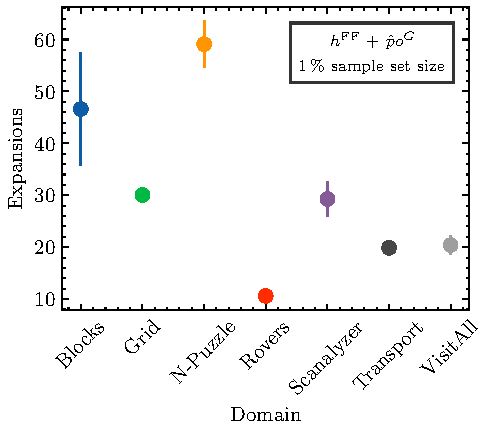
\includegraphics[width=\linewidth]{img/error_hFF_poG_1pct.pdf}
  \end{subfigure}
  %\hfill
  \begin{subfigure}{0.41\textwidth}
    \centering
    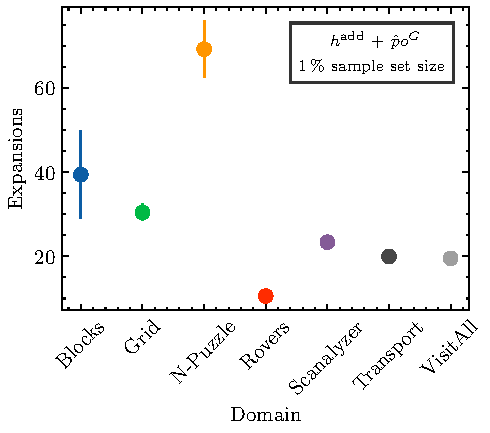
\includegraphics[width=\linewidth]{img/error_hADD_poG_1pct.pdf}
  \end{subfigure}

  \vspace{0.5cm}

  %\hfill
  \begin{subfigure}{0.41\textwidth}
    \centering
    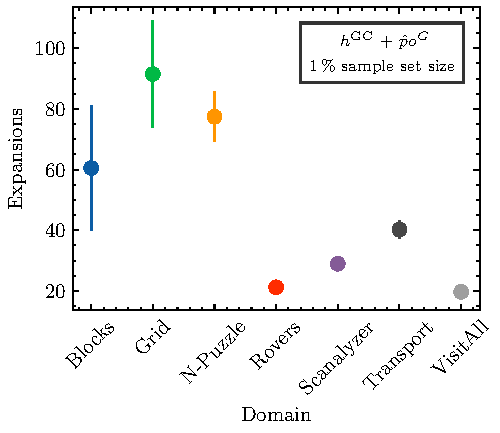
\includegraphics[width=\linewidth]{img/error_hGC_poG_1pct.pdf}
  \end{subfigure}
  \begin{subfigure}{0.41\textwidth}
    \centering
    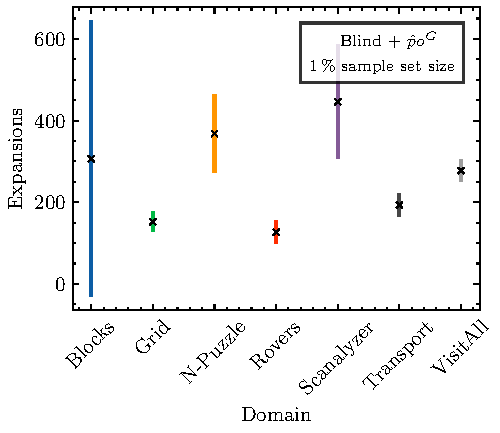
\includegraphics[width=\linewidth]{img/error_blind_poG_1pct.pdf}
  \end{subfigure}
  %\hfill
  \label{fig:errors-logic}
\end{figure}


\chapter{Conclusion}
\label{cha:conclusion}
Researchers have extensively investigated learning heuristic functions for solving planning tasks.
However, in this study, we explored the sampling and learning of preferred operators for the first time.

The findings suggest that learning-based approaches have a considerable potential to outperform logic-based methods. We demonstrate that learned preferred operators can surpass logic-based preferred operators like \poff over the considered planning tasks. Furthermore, the learned preferred operators have fewer expansions than \poff when paired uninformed and less informed heuristics, although further investigation is needed to understand this phenomenon fully.
The experiments highlight the ability to discover preferred operators and train an NN capable of generalizing for the entire task using a subset of the state space. Analysis between successor and predecessor states proved to be an effective method for discovering preferred operators from a limited sample set.

A limitation of learned preferred operators is the number of samples required for training. Our experiments used small state spaces and a relatively simple NN as a first step to explore learning preferred operators. Consequently, we had access to the complete state space of a task. However, this is infeasible for harder tasks, as state spaces tend to grow exponentially as the amount of information needed to describe them increases, meaning that if computational resources are a concern, even sampling $1\,\%$ of the state space can be impractical.
Another problem involves the size of the output tensor, where certain domains have thousands of classes in larger tasks, significantly affecting training efficiency.
Therefore, to improve learning efficiency, future research could focus on experimenting with other learning architectures that enable the generalization of preferred operators using smaller sample sets, or an alternative representation of preferred operators as the output tensor.

Overall, this research presents new opportunities for enhancing heuristic search in planning by using learned preferred operators, highlighting the potential of learning-based methods that require minimal domain logic.

\bibliographystyle{abntex2-alf}
\bibliography{biblio}

\appendix

\chapter{Maximum Regression Depth with \bfsrs}
\label{cha:max_reg_depth}

\cref{tab:regression-limits} shows the maximum regression depth reached ($h$-value) found in samples generated with \bfsrs using different sample set sizes, compared to the longest distance \distfarthest between the goal condition and any potential initial state in the forward state space, and the regression limit $L$ by \citet{Bettker.etal/2022}.

\begin{table}[!h]
\centering
\caption[Maximum regression depth in \bfsrs]{Maximum regression depth found in samples generated with \bfsrs on different sample set sizes, compared with the longest distance \distfarthest and the regression limit $L$.}
\label{tab:regression-limits}
\vspace{\baselineskip}
\begin{tabular}{lrrrrrrrrr}
\toprule
           &     &        & \multicolumn{7}{c}{\bfsrs} \\
\cmidrule(lr){4-10}
Domain     & \distfarthest & $L$ & $1\,\%$ & $5\,\%$   & $10\,\%$ & $20\,\%$ & $30\,\%$ & $40\,\%$ & $50\,\%$ \\
\midrule
Blocks     & 24            & 17  & 20 & 22 & 23 & 24 & 25 & 25 & 26  \\
Grid       & 32            & 44  & 15 & 19 & 21 & 23 & 24 & 24 & 25  \\
N-Puzzle   & 31            & 41  & 21 & 26 & 28 & 31 & 32 & 33 & 34   \\
Rovers     & 19            & 27  & 15 & 18 & 19 & 20 & 20 & 20 & 20   \\
Scanalyzer & 15            & 20  & 10 & 14 & 15 & 16 & 17 & 16 & 17  \\
Transport  & 17            & 35  & 12 & 16 & 17 & 19 & 20 & 20 & 20   \\
VisitAll   & 15            & 17  & 11 & 14 & 16 & 17 & 17 & 18 & 18  \\
\bottomrule
\end{tabular}
\end{table}


\chapter{Tasks of Each Domain}
\label{cha:tasks_each_domain}
The Blocks World domain involves manipulating blocks on a table to achieve a desired configuration through a sequence of actions. We used a planning task with $7$ blocks.

In the Grid domain, an agent capable of holding a key traverses a grid, with certain cells being locked and requiring specific keys to open. We used a planning task with a $4 \times 4$ grid, four locked cells, and three keys with two possible shapes, circle or square.

The N-Puzzle domain consists of a square grid with numbered tiles. The objective is to rearrange the tiles from their initial scrambled state to a desired goal condition. We used a planning task with a $3 \times 3$ grid.

The Rovers domain involves rovers navigating a grid-based environment with missions like exploration or resource gathering. Each rover has specific capabilities and limitations, including movement range, sensing, and interaction abilities. We used a planning task with two rovers, each with one storage capacity and one camera, and four waypoints with different objectives.

The Scanalyzer domain models automated greenhouse logistics, using imaging facilities to collect plant data and conveyor belts to transport plants between smart greenhouses and imaging facilities. We use a planning task with six conveyor belts and six batches of plants.

The Transport domain consists of transporting packages from one location to another using trucks with specific capacities. We use a planning task with nine cities, two trucks, and four packages.

The VisitAll domain consists of a robot that needs to visit all the cells of a grid once. We use a planning task with a $4 \times 4$ grid.

See the tasks in the directory \texttt{tasks/experiments} for more details.

\chapter[Preferred Operators Without Boosting]{Discovered Preferred Operators Without Boosting}
\label{cha:discovered_pos_boost0}
\cref{tab:learning_discovered_pos_boost0} shows the number of expanded states using the discovered preferred operators \pog but no boosting during search, i.e., states are expanded alternately from the default and preferred queues.

\begin{table}[!h]
\centering
\caption[Expansions of \pog without boosting]{Expansions of DQ-GBFS guided by \hnn with \pog trained with the discovered learned operators varying the size of the sample set according to different percentages of the state space size. Boosting is disabled.}
\label{tab:learning_discovered_pos_boost0}
\vspace{\baselineskip}
\begin{tabular}{lrrrrrrr}
\toprule
& \multicolumn{7}{c}{$\pog$} \\
\cmidrule(lr){2-8}
Domain     & $1\,\%$ & $5\,\%$   & $10\,\%$ & $20\,\%$ & $30\,\%$ & $40\,\%$ & $50\,\%$ \\ \midrule
Blocks         & 43.6 & 32.0 & 33.3  & 34.6  & 34.6  & 36.1  & 36.5  \\
Grid           & 63.7 & 55.6 & 47.5  & 35.0  & 31.9  & 31.5  & 30.9  \\
N-Puzzle       & 57.5 & 44.1 & 42.1  & 40.5  & 39.8  & 38.9  & 39.0  \\
Rovers         & 14.0 & 13.4 & 13.5  & 13.3  & 13.3  & 13.3  & 13.3  \\
Scanalyzerunit & 31.1 & 21.6 & 17.2  & 16.1  & 16.0  & 15.8  & 16.3  \\
Transportunit  & 22.4 & 19.7 & 19.3  & 19.1  & 18.7  & 18.6  & 18.4  \\
VisitAll       & 20.0 & 18.9 & 18.2  & 18.2  & 18.0  & 18.1  & 18.6  \\ \midrule
Geo. mean      & 31.6 & 26.2 & 24.6  & 23.2  & 22.7  & 22.7  & 22.9 \\ \bottomrule
\end{tabular}
\end{table}


\chapter{\bfsrs with different values of $k$}
\label{cha:bfsss_pct}

\cref{tab:bfsss_pct} shows the number of expanded states of \pog trained on sample sets with varying $k_{1}$, i.e., number of samples generated by BFS in the first phase of \bfsrs. The values of $k_{1}$ used are $0.05$, $0.1$, $0.2$, $0.3$, $0.4$, $0.5$, and $0.6$. Note that $k_{2} = 1 - k_{1}$.

\begin{table}[!h]
\centering
\caption[Expansions of \pog with varying values of $k_{1}$]{Expansions of GBFS guided by \hnn with \pog on $1\,\%$ sample set size, with varying number of samples generated by BFS ($k_{1}$) in the first phase of \bfsrs.}
\label{tab:bfsss_pct}
\vspace{\baselineskip}
\begin{tabular}{lrrrrrrrr}
\toprule
& \multicolumn{7}{c}{$\pog$} \\
\cmidrule(lr){2-8}
Domain     & $0.05$ &$0.1$ & $0.2$   & $0.3$ & $0.4$ & $0.5$ & $0.6$ \\ \midrule
Blocks     & 38.9   & 43.0  & \textbf{42.9}  & 45.2  & 48.9  & 54.5  & 54.6  \\
Grid       & 72.0   & \textbf{67.4}  & 77.0  & 77.0  & 79.1  & 79.0  & 81.6  \\
N-Puzzle   & 57.2   & 53.3  & \textbf{49.5}  & 53.8  & 51.8  & 51.2  & 52.6  \\
Rovers     & \textbf{12.0}   & 12.2  & 12.3  & 12.2  & \textbf{12.0}  & \textbf{12.0}  & 12.1  \\
Scanalyzer & 31.9   & \textbf{30.7}  & 31.8  & 32.5  & 31.3  & 32.6  & 31.4  \\
Transport  & 22.0   & \textbf{21.4}  & 21.5  & 22.0  & 21.6  & \textbf{21.4}  & 21.6  \\
VisitAll   & 21.4   & 20.5  & 19.8  & 20.2  & 20.1  & \textbf{19.3}  & 19.9  \\ \midrule
Geo. mean  & 31.2   & \textbf{30.6}  & 31.0  & 31.8  & 31.8  & 32.2  & 32.5  \\ \bottomrule
\end{tabular}
\end{table}


\chapter{Training Details}
\label{cha:training_details}

\cref{tab:training_info_hnn} presents the mean training information for the regression networks used to learn the heuristic~\hnn across $25$ different seed runs for each task, trained over $1\,\%$ sample set size. The table shows the epoch associated with the minimum validation loss, the value of the minimum validation loss, and the elapsed time required to train the NN.~\cref{tab:training_info} has the same information, but for learning~\pog with classification networks using varied sample set sizes, and also showing the number of preferred operators per sample. All the networks early-stopped.

\begin{table}[!h]
\centering
%\small
%\setlength{\tabcolsep}{0.7ex}
\caption{Training summary over $25$ seeds for each domain, with the goal of learning \pog.} 
\label{tab:training_info}
\vspace{\baselineskip}
\scalebox{0.85}{
\begin{tabular}{lrrrrr}
\toprule
Domain   & Sample set size ($\%$) &  Best epoch &  Val. loss &  Elapsed time (s) &  \# ops./sample \\
\midrule
Blocks   & 1 &       167.9 &      0.0113 &                16.8 &                           1.1 \\
         & 5 &        75.0 &      0.0130 &                53.9 &                           1.2 \\
         & 10 &        52.9 &      0.0118 &                92.9 &                           1.2 \\
         & 20 &        42.2 &      0.0104 &               174.2 &                           1.3 \\
         & 30 &        38.6 &      0.0092 &               252.3 &                           1.3 \\
         & 40 &        39.0 &      0.0083 &               342.7 &                           1.4 \\
         & 50 &        35.4 &      0.0076 &               415.6 &                           1.4 \\ \midrule
Grid     & 1 &       105.5 &      0.0022 &                99.2 &                           1.2 \\
         & 5 &        53.1 &      0.0018 &               378.4 &                           1.3 \\
         & 10 &        45.3 &      0.0016 &               730.3 &                           1.3 \\
         & 20 &        39.2 &      0.0014 &              1448.1 &                           1.3 \\
         & 30 &        35.8 &      0.0013 &              2079.7 &                           1.3 \\
         & 40 &        34.3 &      0.0012 &              2758.8 &                           1.3 \\
         & 50 &        34.5 &      0.0011 &              3449.9 &                           1.3 \\ \midrule
N-Puzzle & 1 &       115.0 &      0.0101 &                39.6 &                           1.0 \\
         & 5 &        57.9 &      0.0069 &               145.5 &                           1.0 \\
         & 10 &        48.6 &      0.0070 &               273.3 &                           1.1 \\
         & 20 &        47.9 &      0.0069 &               557.3 &                           1.1 \\
         & 30 &        44.8 &      0.0069 &               811.0 &                           1.1 \\
         & 40 &        42.8 &      0.0070 &              1093.8 &                           1.1 \\
         & 50 &        39.3 &      0.0070 &              1325.7 &                           1.1 \\ \midrule
Rovers   & 1 &        30.6 &      0.0756 &                62.8 &                           2.1 \\
         & 5 &        24.7 &      0.0735 &               305.7 &                           2.9 \\
         & 10 &        22.8 &      0.0678 &               609.4 &                           3.3 \\
         & 20 &        27.8 &      0.0619 &               966.3 &                           3.4 \\
         & 30 &        27.4 &      0.0618 &               969.2 &                           3.4 \\
         & 50 &        28.2 &      0.0618 &               986.9 &                           3.4 \\ \midrule
Scanalyzer & 1 &       186.9 &      0.0244 &                15.2 &                           1.8 \\
         & 5 &       111.4 &      0.0158 &                54.8 &                           2.5 \\
         & 10 &       107.7 &      0.0133 &               105.6 &                           2.9 \\
         & 20 &       109.7 &      0.0131 &               213.7 &                           3.3 \\
         & 30 &       109.9 &      0.0130 &               323.0 &                           3.6 \\
         & 40 &       110.8 &      0.0132 &               441.9 &                           3.8 \\
         & 50 &       115.0 &      0.0131 &               554.3 &                           4.1 \\ \midrule
Transport & 1 &        80.6 &      0.0041 &               170.6 &                           1.3 \\
         & 5 &        45.7 &      0.0035 &               694.8 &                           1.4 \\
         & 10 &        40.3 &      0.0036 &              1326.4 &                           1.4 \\
         & 20 &        39.6 &      0.0035 &              2728.8 &                           1.4 \\
         & 30 &        39.4 &      0.0036 &              3974.5 &                           1.5 \\
         & 40 &        40.1 &      0.0036 &              5404.9 &                           1.5 \\
         & 50 &        41.0 &      0.0036 &              6433.7 &                           1.5 \\ \midrule
VisitAll & 1 &       196.8 &      0.0258 &                21.8 &                           1.4 \\
         & 5 &       105.7 &      0.0319 &                72.5 &                           1.5 \\
         & 10 &        84.9 &      0.0335 &               130.1 &                           1.5 \\
         & 20 &        75.2 &      0.0339 &               242.3 &                           1.6 \\
         & 30 &        69.5 &      0.0338 &               355.1 &                           1.7 \\
         & 40 &        73.3 &      0.0337 &               431.1 &                           1.7 \\
         & 50 &        74.0 &      0.0333 &               540.4 &                           1.8 \\
\bottomrule
\end{tabular}
}
\end{table}


\chapter{Resumo Expandido}
\noindent
%\textbf{Resolução 02/2021 -- Redação de Teses e Dissertações em Inglês}
%Dissertações de Mestrado e Teses de Doutorado do PPGC, bem como outros
%trabalhos escritos tais como Proposta de Tese e PEP, poderão ser
%redigidas em inglês desde que contenham um título e resumo expandido
%redigidos em português. O resumo expandido deve conter no mínimo duas
%páginas inteiras, deve aparecer como apêndice e deve conter as
%principais contribuições e resultados do trabalho.

No contexto de tarefas de planejamento, os agentes precisam a selecionar a melhor ação possível dentre um conjunto consideravelmente vasto de opções disponíveis em cada etapa. Planejadores lógicos têm sido usados para lidar com esse problema, aplicando operadores preferidos que reduzem significativamente a quantidade de ações a serem consideradas. Os planejadores lógicos que incorporam operadores preferidos na busca foram os vencedores da trilha \emph{satisficing} da \emph{International Planning Competition} (IPC) em 2004~\cite{Helmert/2006}, 2008~\cite{Richter.lama.etal/2010}, 2011~\cite{Richter.lama.etal/2011}, and 2018~\cite{Seipp-fast.etal/2018}.
No entanto, este trabalho apresenta um método que vai além dessas abordagens convencionais, introduzindo uma estratégia de amostragem e aprendizado de operadores preferidos com o objetivo de generalização em todo o espaço de estados de uma tarefa de planejamento.

O objetivo principal deste trabalho é identificar os operadores preferidos ideais, que se encontram nos caminhos mais curtos que levam a um objetivo específico. O desafio reside no fato de que os espaços de estado geralmente são extremamente grandes, o que dificulta a exploração completa de todas as possibilidades. Para contornar essa limitação, desenvolvemos uma nova abordagem de amostragem adaptada, projetada para extrair operadores preferidos de alta qualidade de um conjunto de amostras que representa uma fração do espaço de estados completo. Os resultados demonstraram que essa abordagem reduzida ainda é capaz de alcançar excelentes desempenhos nas tarefas de planejamento consideradas.

Para fornecer uma análise mais abrangente dessa nova categoria de operadores preferidos, realizamos experimentos controlados em tarefas com espaços de estados pequenos, onde conseguimos estimativas perfeitas para o goal. Comparamos sistematicamente os resultados da abordagem proposta com os operadores preferidos do Fast-Forward (FF)~\cite{Hoffmann.Nebel/2001, Helmert/2006}, avaliamos a eficácia dos operadores preferidos aprendidos em diversos tamanhos de amostra e exploraramos seu desempenho ao serem combinados com diferentes funções heurísticas. Essa investigação detalhada permite uma compreensão mais profunda das vantagens e limitações dos operadores preferidos aprendidos.

Este estudo representa a primeira tentativa de descobrir operadores preferidos a partir de um conjunto de amostras e usar uma NN para aprendê-los. Apresentamos um novo método de amostragem e uma nova técnica para identificar operadores preferidos em amostras. A técnica de amostragem envolve regressão do estado objetivo, construindo um grafo com estados amostrados que representam suas relações sucessor-predecessor e determinando, para cada estado, o conjunto de operadores usados para atingir o estado objetivo no menor caminho como operadores preferidos. Este estudo revela que uma rede neural pode aprender os operadores preferidos a partir de um subconjunto do espaço de estados e estender esse aprendizado de forma eficaz no espaço de estados em diversos domínios de planejamento. A abordagem proposta supera o melhor método atual de operadores preferidos do FF nas tarefas de referência. Em particular, este trabalho apresenta:

\begin{itemize}
\item Um novo método de amostragem adaptado para descobrir operadores preferidos.
\item Um novo método baseado em grafos de caminho mais curto para descobrir operadores preferidos em um conjunto de amostras existente.
\item Uma análise da qualidade dos operadores preferidos aprendidos e uma comparação com os operadores preferidos do FF.
\end{itemize}

Um exemplo de resultado consiste em uma rede treinada sobre uma quantidade de amostras equivalente a $5\,\%$ do espaço de estados completo de uma tarefa. Nesse caso, os operadores preferidos aprendidos superam significativamente uma busca guiada apenas por uma heurística aprendida, com diminuição de $36\,\%$ em número de estados expandidos. Além disso, eles também superam os operadores do FF em média, com aproximadamente $20\,\%$ de expansões a menos.

\end{document}
